

\section{An\'alisis}

En esta secci\'on presentaremos el an\'alisis de los distintos casos de estudio abordados. Cada subsecci\'on corresponder\'a a uno de ellos, abord\'andolos de menor a mayor tamaño.

\subsection{Red dom\'estica}

\subsubsection{Nodos intervinientes}


\begin{figure}[h!]
    \centering                                                       
    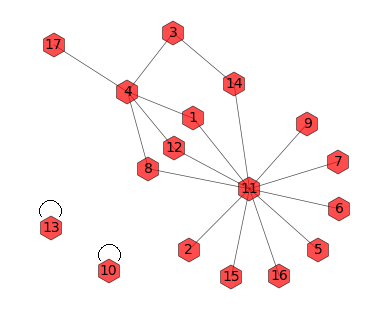
\includegraphics[width=400pt]{img/domesticaGraph.png}
    \caption{Grafo de Red Doméstica}
    \label{domesticaGraph}
\end{figure}


\subsubsection{Frecuencia de los distintos tipos de paquetes}

En el gr\'afico \ref{domesticaPaquetes} se pueden ver los resultados de obtenidos.

\begin{figure}[h!]
    \centering                                                       
    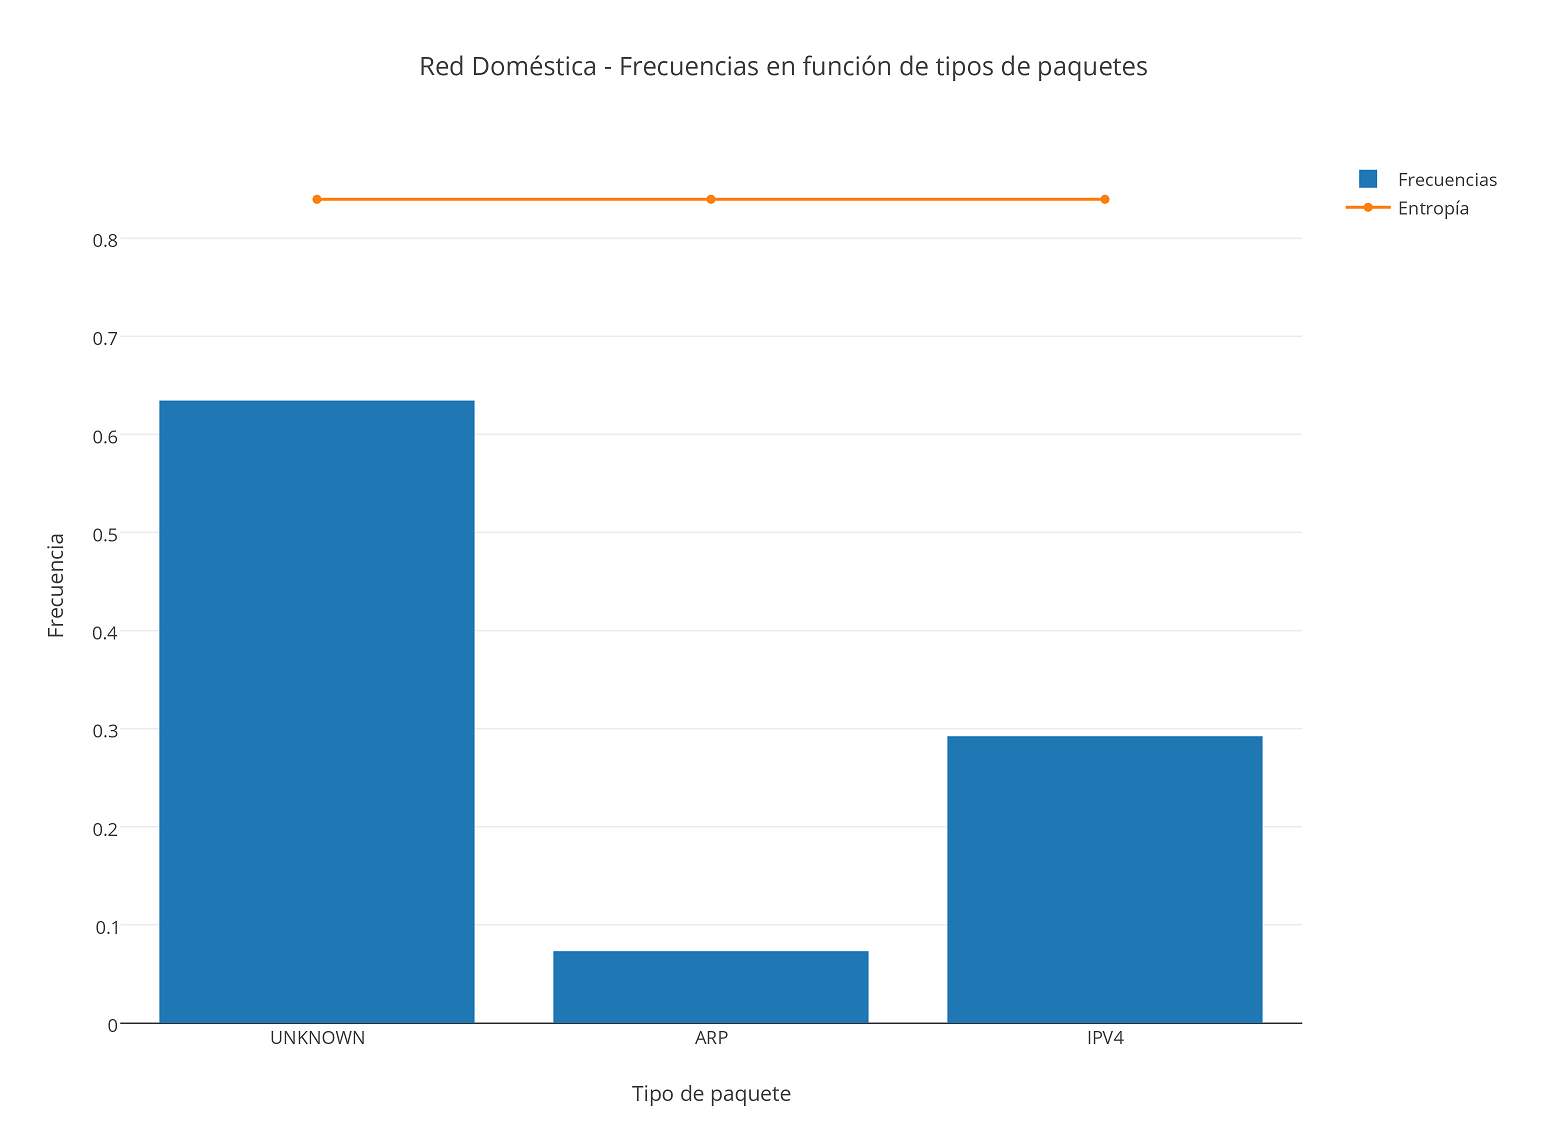
\includegraphics[width=400pt]{img/DomesticaFrecuenciaVsTipoPaquetes}
    \caption{}
    \label{domesticaPaquetes}
\end{figure}


En la red analizada exist\'ian dos m\'aquinas conectadas por cable al router y el resto estaban enlazados al mismo utilizando el wifi, entre ellos la computadora en la cual se ejecut\'o el algoritmo de captura de paquetes. Esto podr\'ia explicar la presencia de dos redes en las mediciones, una de ellas (169.254) es la red formada por las dos computadoras enlazadas por cable y el proxy que se comunica con internet y la otra red (192.168.0) es la conformada por los dispositivos WiFi. Si esto es cierto el 169.254.93.30 podr\'ia ser el proxy y el 192.168.0.1 el nodo que rutea a los dispositivos de la red de wifi a la red del proxy.\\
El grafo muestra que el IP 0.0.0.0 (nodo 4) tuvo contacto con cinco nodos. Puntualmente El 0.0.0.0 envi\'o datos a cuatro nodos cuyos IP tuvieron actividad con otros nodos de la red, con lo cual se puede deducir esos mensajes provenian de los dispositivos reporesentados por esos cuatro nodos, que intentaban determinar si exist\'ian duplicados de su IP en la red. \\
El nodo 169.254.93.30 es el \'unico env\'ia paquetes al 0.0.0.0, lo cual puede tratarse de un mecanismo de IP para enviar informaci\'on a todas las redes.\\
\subsubsection{Informaci\'on de las fuentes emisoras y receptoras de paquetes ARP.}

Para realizar este caso comparamos la informaci\'on proporcionada por las fuentes emisoras de paquetes ARP e ilustramos asimismo la entrop\'ia de la fuente. Los resultados se pueden observar en los gr\'aficos \ref{domesticaEmisoras} y \ref{domesticaReceptoras}

\begin{figure}[h!]
    \centering                                                       
    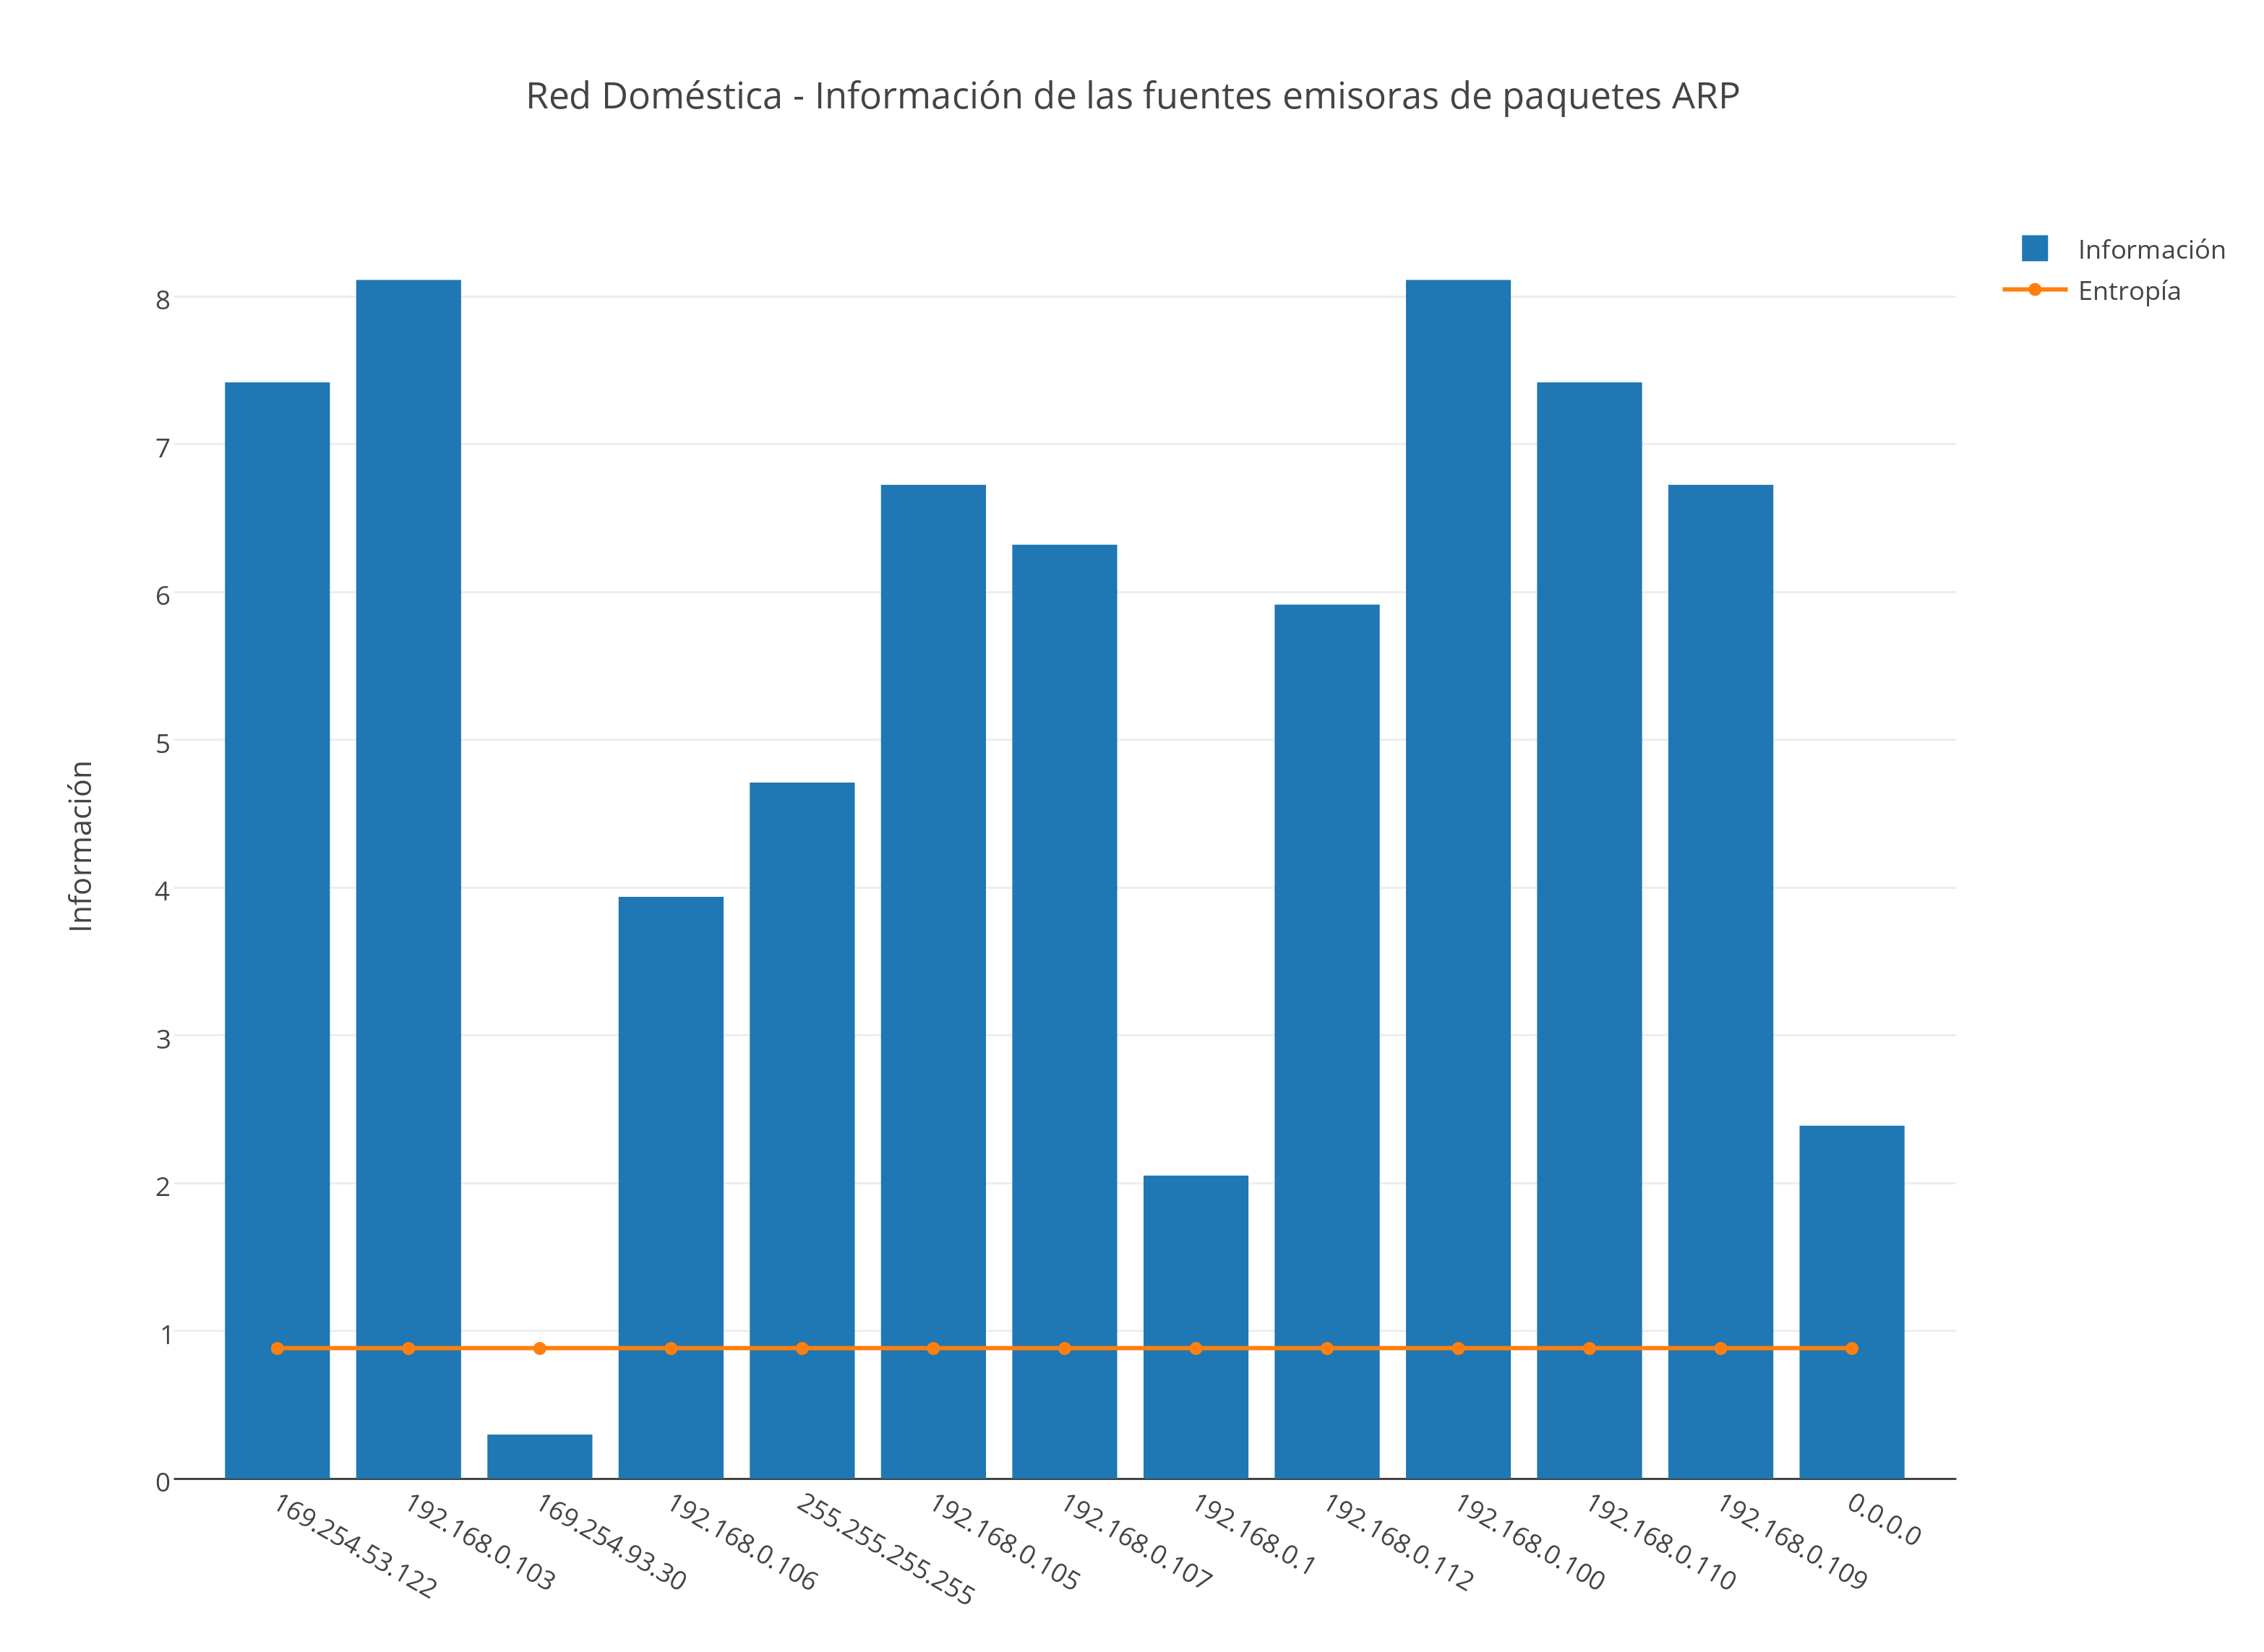
\includegraphics[width=400pt]{img/RedDomesticaFuentesEmisorasARP}
    \caption{}
    \label{domesticaEmisoras}
\end{figure}

En el primero de ellos se ve que existe una \'unica fuente situada por debajo de la entrop\'ia y corresponde a la IP 169.254.93.30. La baja informaci\'on que aporta indica que se trata de un nodo que emite muchos paquetes ARP. En contraposici\'on, las IP 192.168.0.103 y 192.168.0.100 muestran un gran aporte de informaci\'on, de lo cual se deduce que es poco com\'un que las mismas env\'ien paquetes de solicitud ARP.


\begin{figure}[h!]
    \centering                                                       
    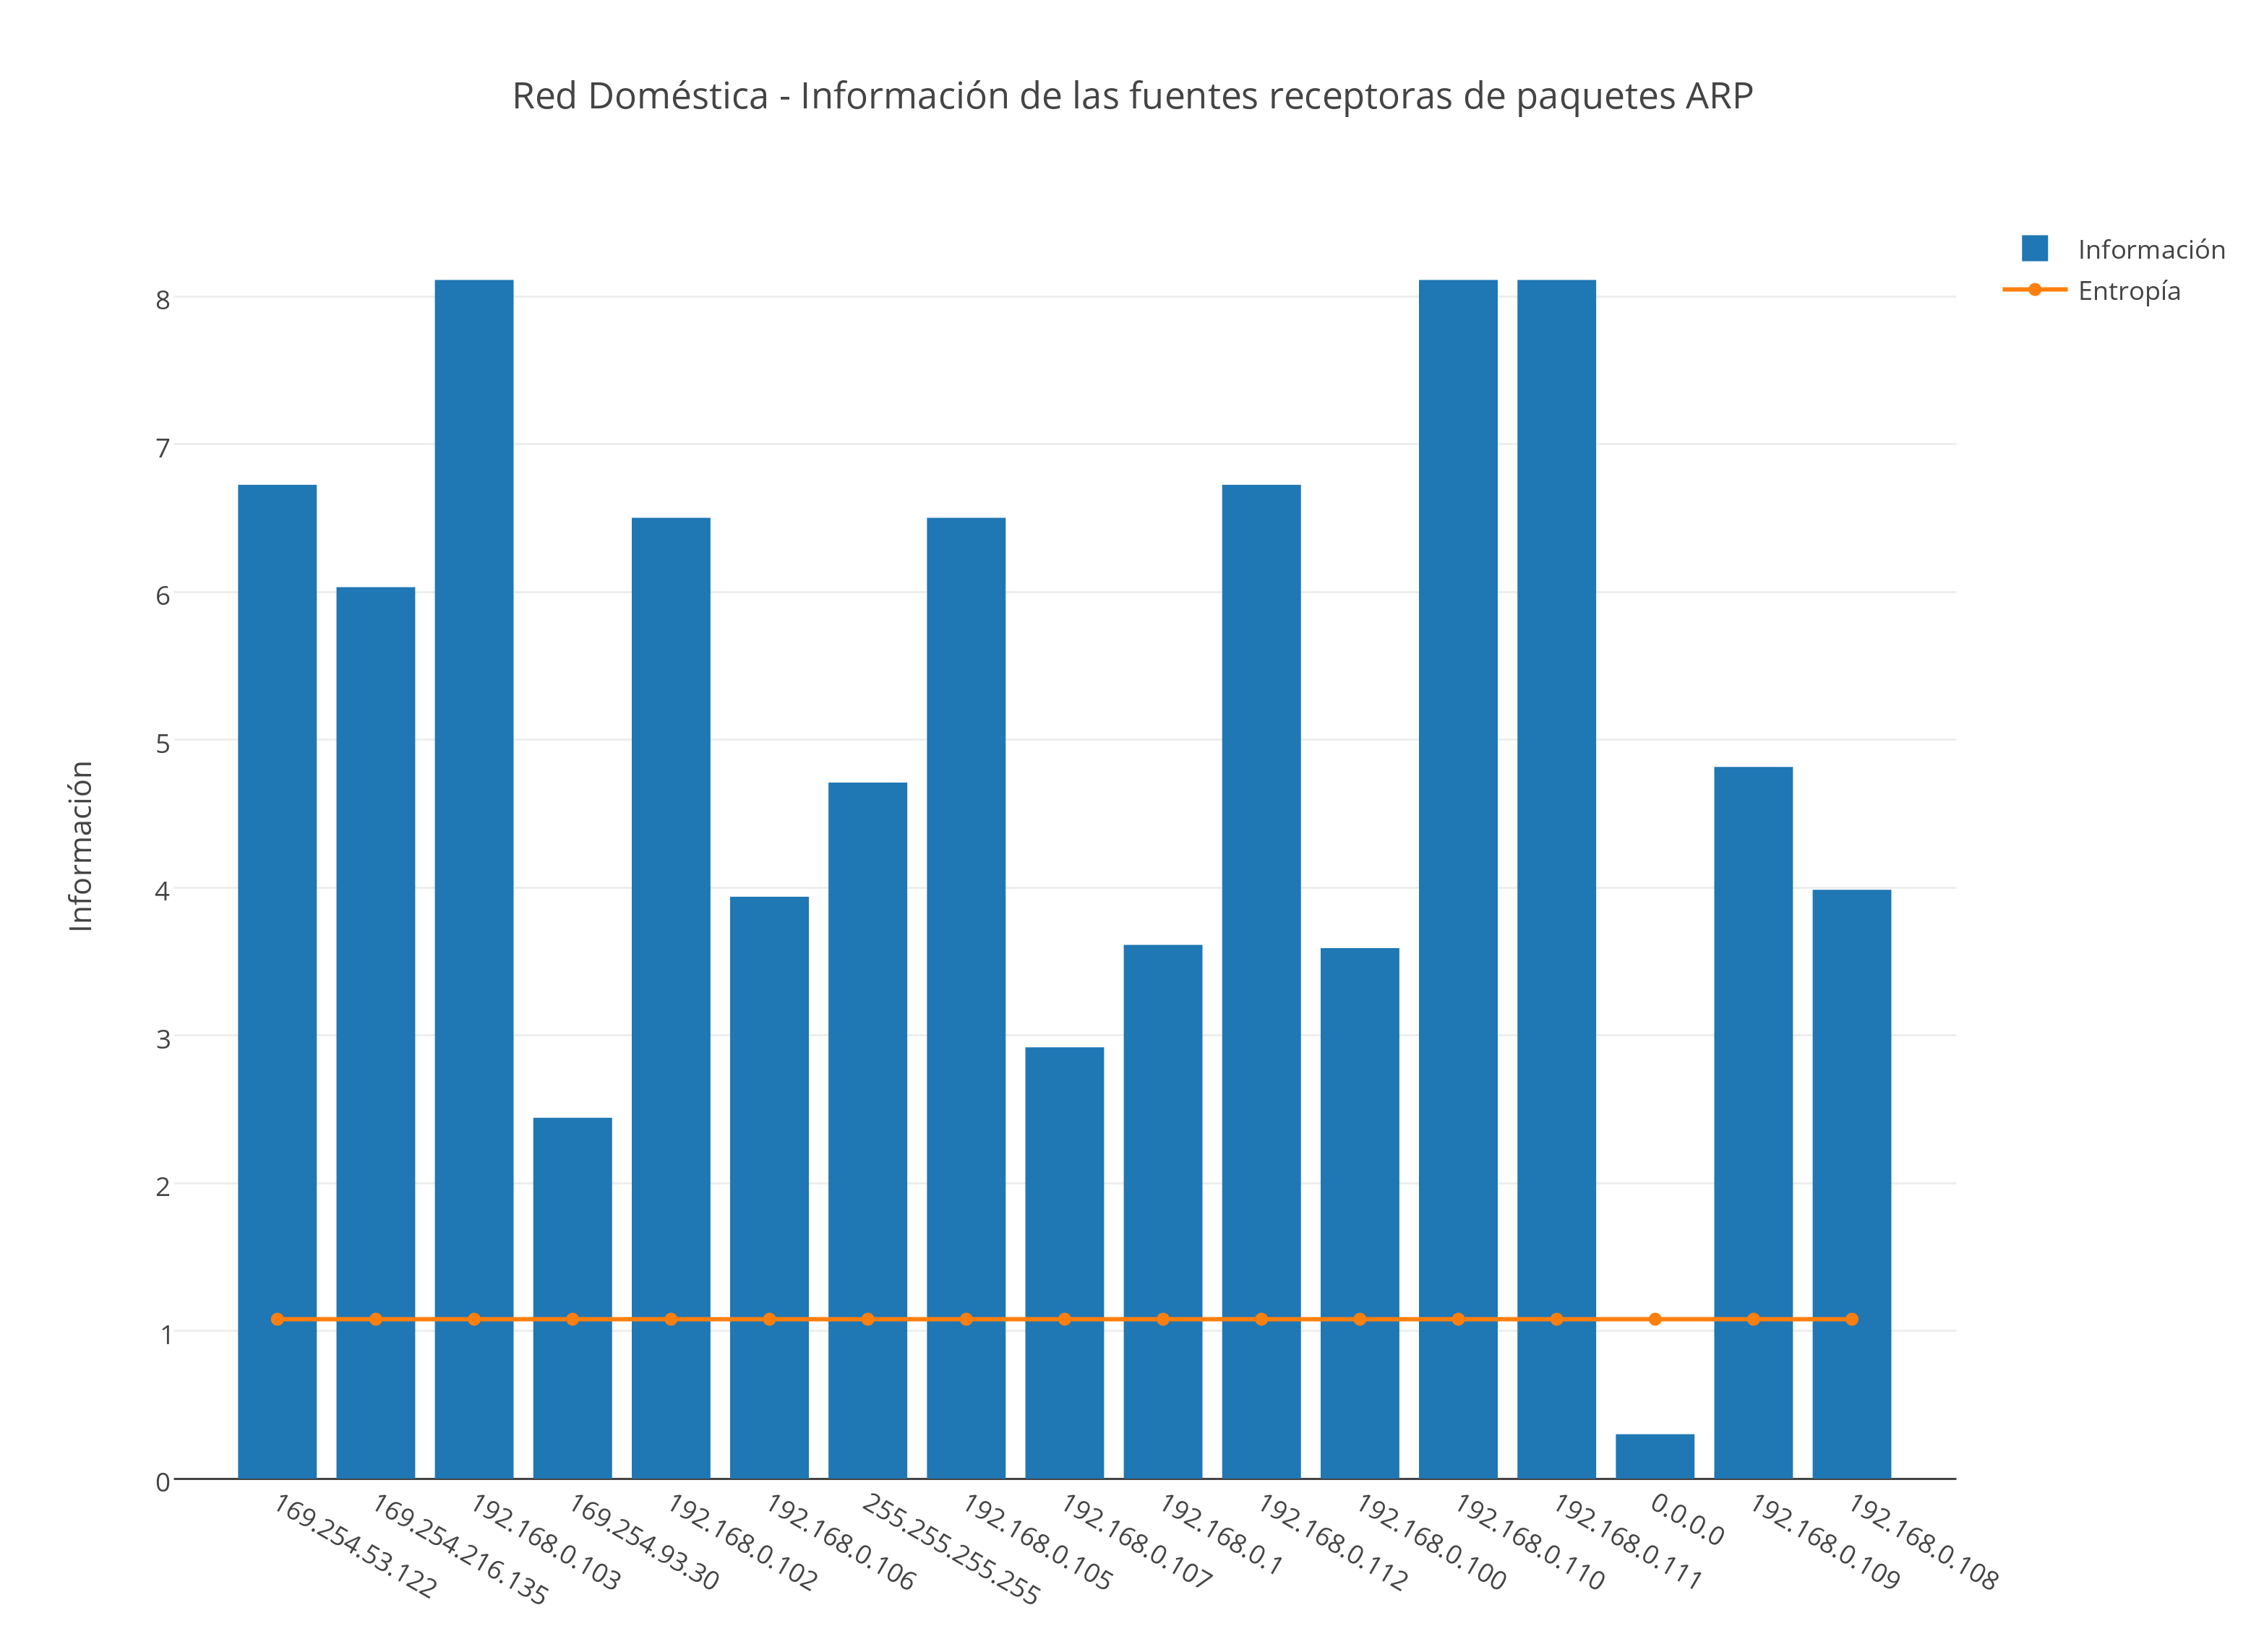
\includegraphics[width=400pt]{img/RedDomesticaFuentesReceptorasARP}
    \caption{}
    \label{domesticaReceptoras}
\end{figure}

En el segundo gr\'afico se observa una entrop\'ia mayor. De esto podr\'ia deducirse que es una fuente a\'un m\'as aleatoria y menos predecible que la que filtra \'unicamente los env\'ios de paquetes ARP.\\
En este caso, los nodos distinguidos son - por su gran valor de informaci\'on - los que mapean las direcciones IP 192.168.0.103, 192.168.0.9 y 192.168.0.111 y, por su poca cantidad de informaci\'on el nodo 0.0.0.0, seguido del 169.254.93.30. Esto indica que frecuentemente se realizan requests a estos \'ultimos hosts, mientras que los primeros son ignorados la mayor parte del tiempo. \\

Por qu\'e es tan frecuente que se realicen solicitudes al host cuya IP es 0.0.0.0? Podr\'iamos pensar que se trata de comunicaciones que un nodo env\'ia a s\'i mismo pero tambi\'en cabr\'ia suponer - de acuerdo a lo investigado - que puede tratarse de un mecanismo de chequeo de IP's duplicadas en la red.\\

Comparando ambos gr\'aficos podr\'iamos decir que es bastante com\'un que la IP 169.254.93.30 env\'ie y reciba paquetes ARP. Es por eso que consideramos que podr\'ia ser un potencial candidato a Router.

Viendo otros datos calculados, observamos que el muestreo de la red detect\'o un alto \'indice de pedidos de direcci\'on por parte del dispositivo con IP 192.168.0.1, el cual contact\'o a varios dispositivos en m\'ultiples ocasiones. Puntualmente, se destac\'o el dispositivo con la IP 192.168.0.107, en el cu\'al hubo 180 solicitudes, contra una 6 solicitudes por parte del 192.168.0.107 al 192.168.0.1.

Por otro lado los dispositivos con la IP 192.168.0.106 y 192.168.0.108 enviaron una alta cantidad de solicitudes al  192.168.0.1 (respecto de la media).

Viendo esto, podemos decir que el dispositivo con IP 192.168.0.1 es un nodo importante en la red, por lo cual pensamos que puede ser otro candidato a ser el Router. Se puede deducir que durante un periodo prolongado el dispositivo 192.168.0.107 estuvo extrayendo informaci\'on del nodo, lo cual explicar\'ia por qu\'e existe un trafico de paquetes m\'as elevado desde el nodo hasta el  192.168.0.107 que desde este \'ultimo al nodo..

En el caso del dispositivo con IP 192.168.0.106, y 192.168.0.108 las solicitudes para buscar al nodo podr\'ian deberse a que estos estaban enviando informaci\'on al nodo.

La mayor\'ia de los dispositivos conten\'ia una IP con el prefijo de 192.168.0, con lo cual se puede deducir que \'esta es la IP de la red analizada. Adem\'as, se han detectado paquetes provenientes de redes privadas distintas (puntualmente de tres dispositivos).

Se registr\'o un trafico m\'inimo entre dispositivos en donde el 192.168.0.1 no estuvo involucrado.


\newpage
\subsection{Red Laboral}

En este segundo caso, se analiz\'o una red laboral de una PyME. La captura se realiz\'o por un lapso de media hora en modo promiscuo.

\subsubsection{Nodos intervinientes}
En el gr\'afico \ref{laboralGraph} se pueden ver los resultados de obtenidos.

\begin{figure}[h!]
    \centering                                                       
    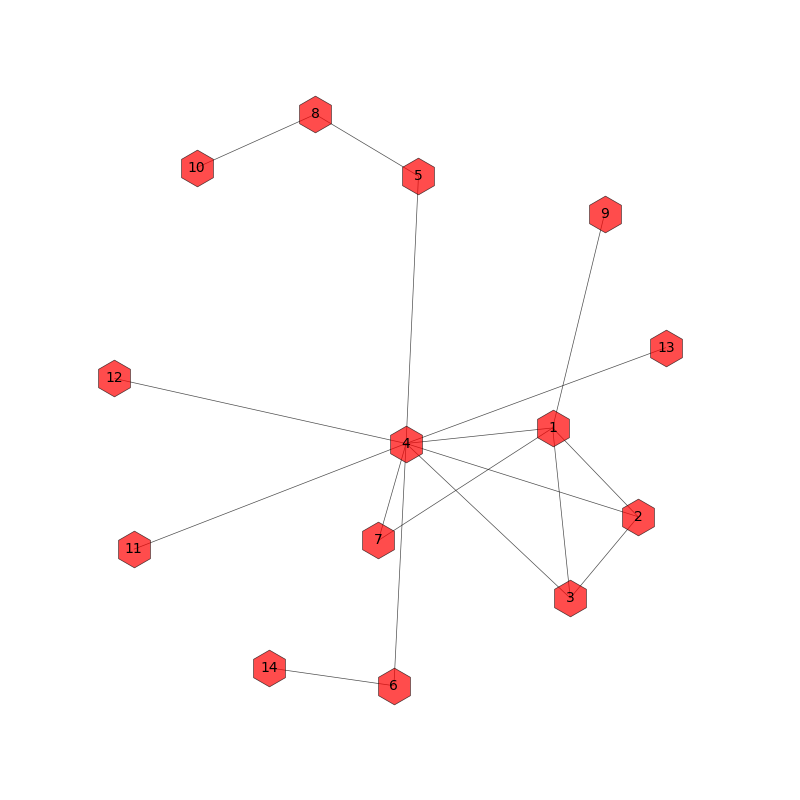
\includegraphics[width=400pt]{img/laboralGraph.png}
    \caption{Grafo de Red Laboral}
    \label{laboralGraph}
\end{figure}

La visualizaci\'on del grafo indicar\'ia, a primera vista, que el nodo 4 se transmite paquetes con la mayor\'ia de los dem\'as v\'ertices (excepto casos particulares) siendo el candidato ideal para ser el router de esta conexi\'on - es decir, el nodo con salida exterior.\\

El nodo 1 tambi\'en se comunica con varios nodos a la vez - esto se debe a que es un servidor local en la oficina, al cual le llegan peticiones de nodos particulares - que a su vez tambi\'en se comunican con los otros que acceden a dicho servidor local. Es decir, el nodo 2, 3, 7 y 9 acceden al servidor local 4, pero a su vez entre el 2 y el 3 se comunican entre ellos.\\

Los nodos 10, 8 y 14 parecieran ser nodos particulares que no se conectan con el router. En particular, el nodo 8 es 0.0.0.0, por lo que en realidad es el nodo 5 y 10 comunic\'andose con ellos mismos . El nodo 14 es una IP interna as\'i que posiblemente es un nodo comunic\'andose con una interfaz propia.\\

Luego de ese an\'alisis, consultamos las IPs con la configuraci\'on de la red (a la que tenemos acceso por ser la red de la oficina laboral). Efectivamente, el nodo 4 es el router, as\'i como el nodo 1 el servidor local estimado, y los nodos 2, 3, 7 y 9 los que se comunican con dicho servidor.\\

La incertidumbre del nodo 14 se resolvi\'o como una Virtual Network Adapter, producto de una Virtual Box corriendo en el nodo 6.\\

Todas las dem\'as relaciones parecen ser naturales, de nodos que se comunican con el router para poder salir a internet.\\

\subsubsection{Frecuencia de los distintos tipos de paquetes}

En el gr\'afico \ref{laboralPaquetes} se pueden ver los resultados de obtenidos. All\'i se observa la predominancia de los paquetes de tipo IPV4. Esto tiene sentido, puesto que en este contexto es m\'as frecuente el intercambio de paquetes a nivel de Internet que el realizado a nivel de la intranet, con la cual las computadoras se encuentran conectadas a trav\'es de Ethernet. Esto tambi\'en considerando que las mediciones fueron realizadas en un momento de mucha actividad de pasaje de paquetes en la red.\\

\begin{figure}[h!]
    \centering                                                       
    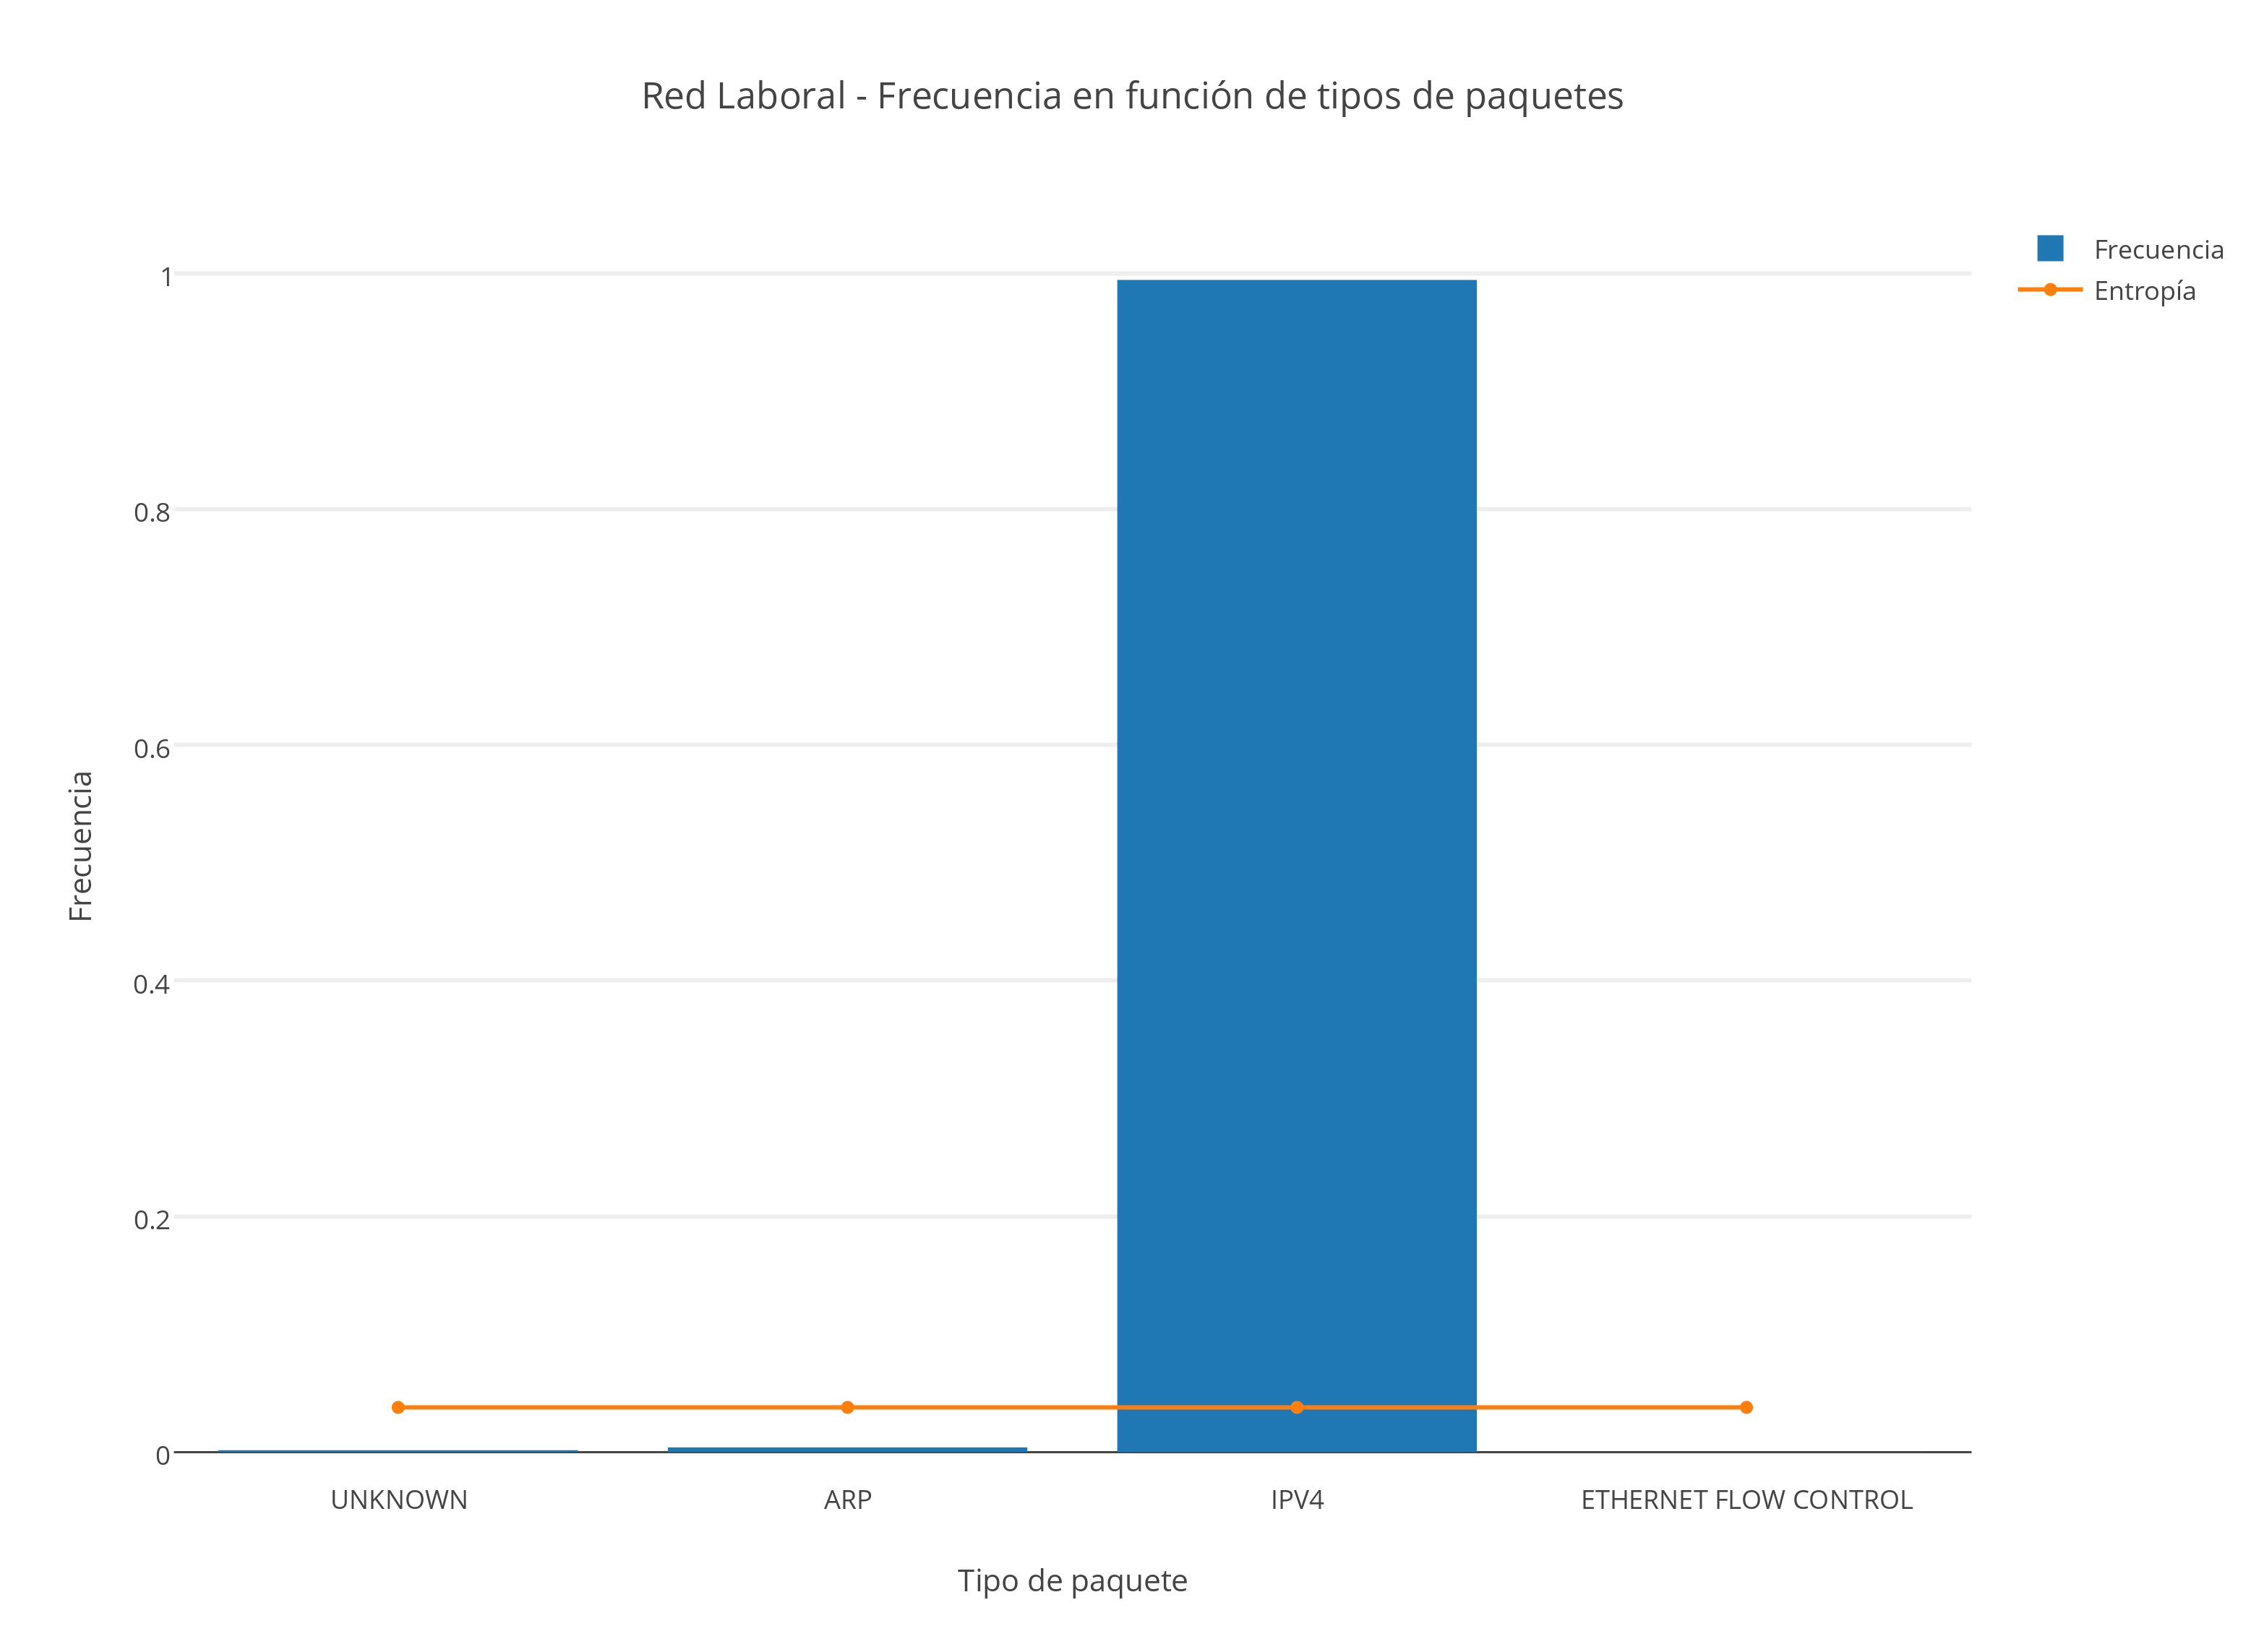
\includegraphics[width=400pt]{img/LaboralFrecuenciaVsTipoPaquetes}
    \caption{}
    \label{laboralPaquetes}
\end{figure}

Comparando las figuras \ref{laboralEmisoras} y \ref{laboralReceptoras} se puede ver que las fuentes receptoras superan en cantidad a las fuentes emisoras.\\

\subsubsection{Informaci\'on de las fuentes emisoras y receptoras de paquetes ARP.}

\begin{figure}[h!]
    \centering                                                       
    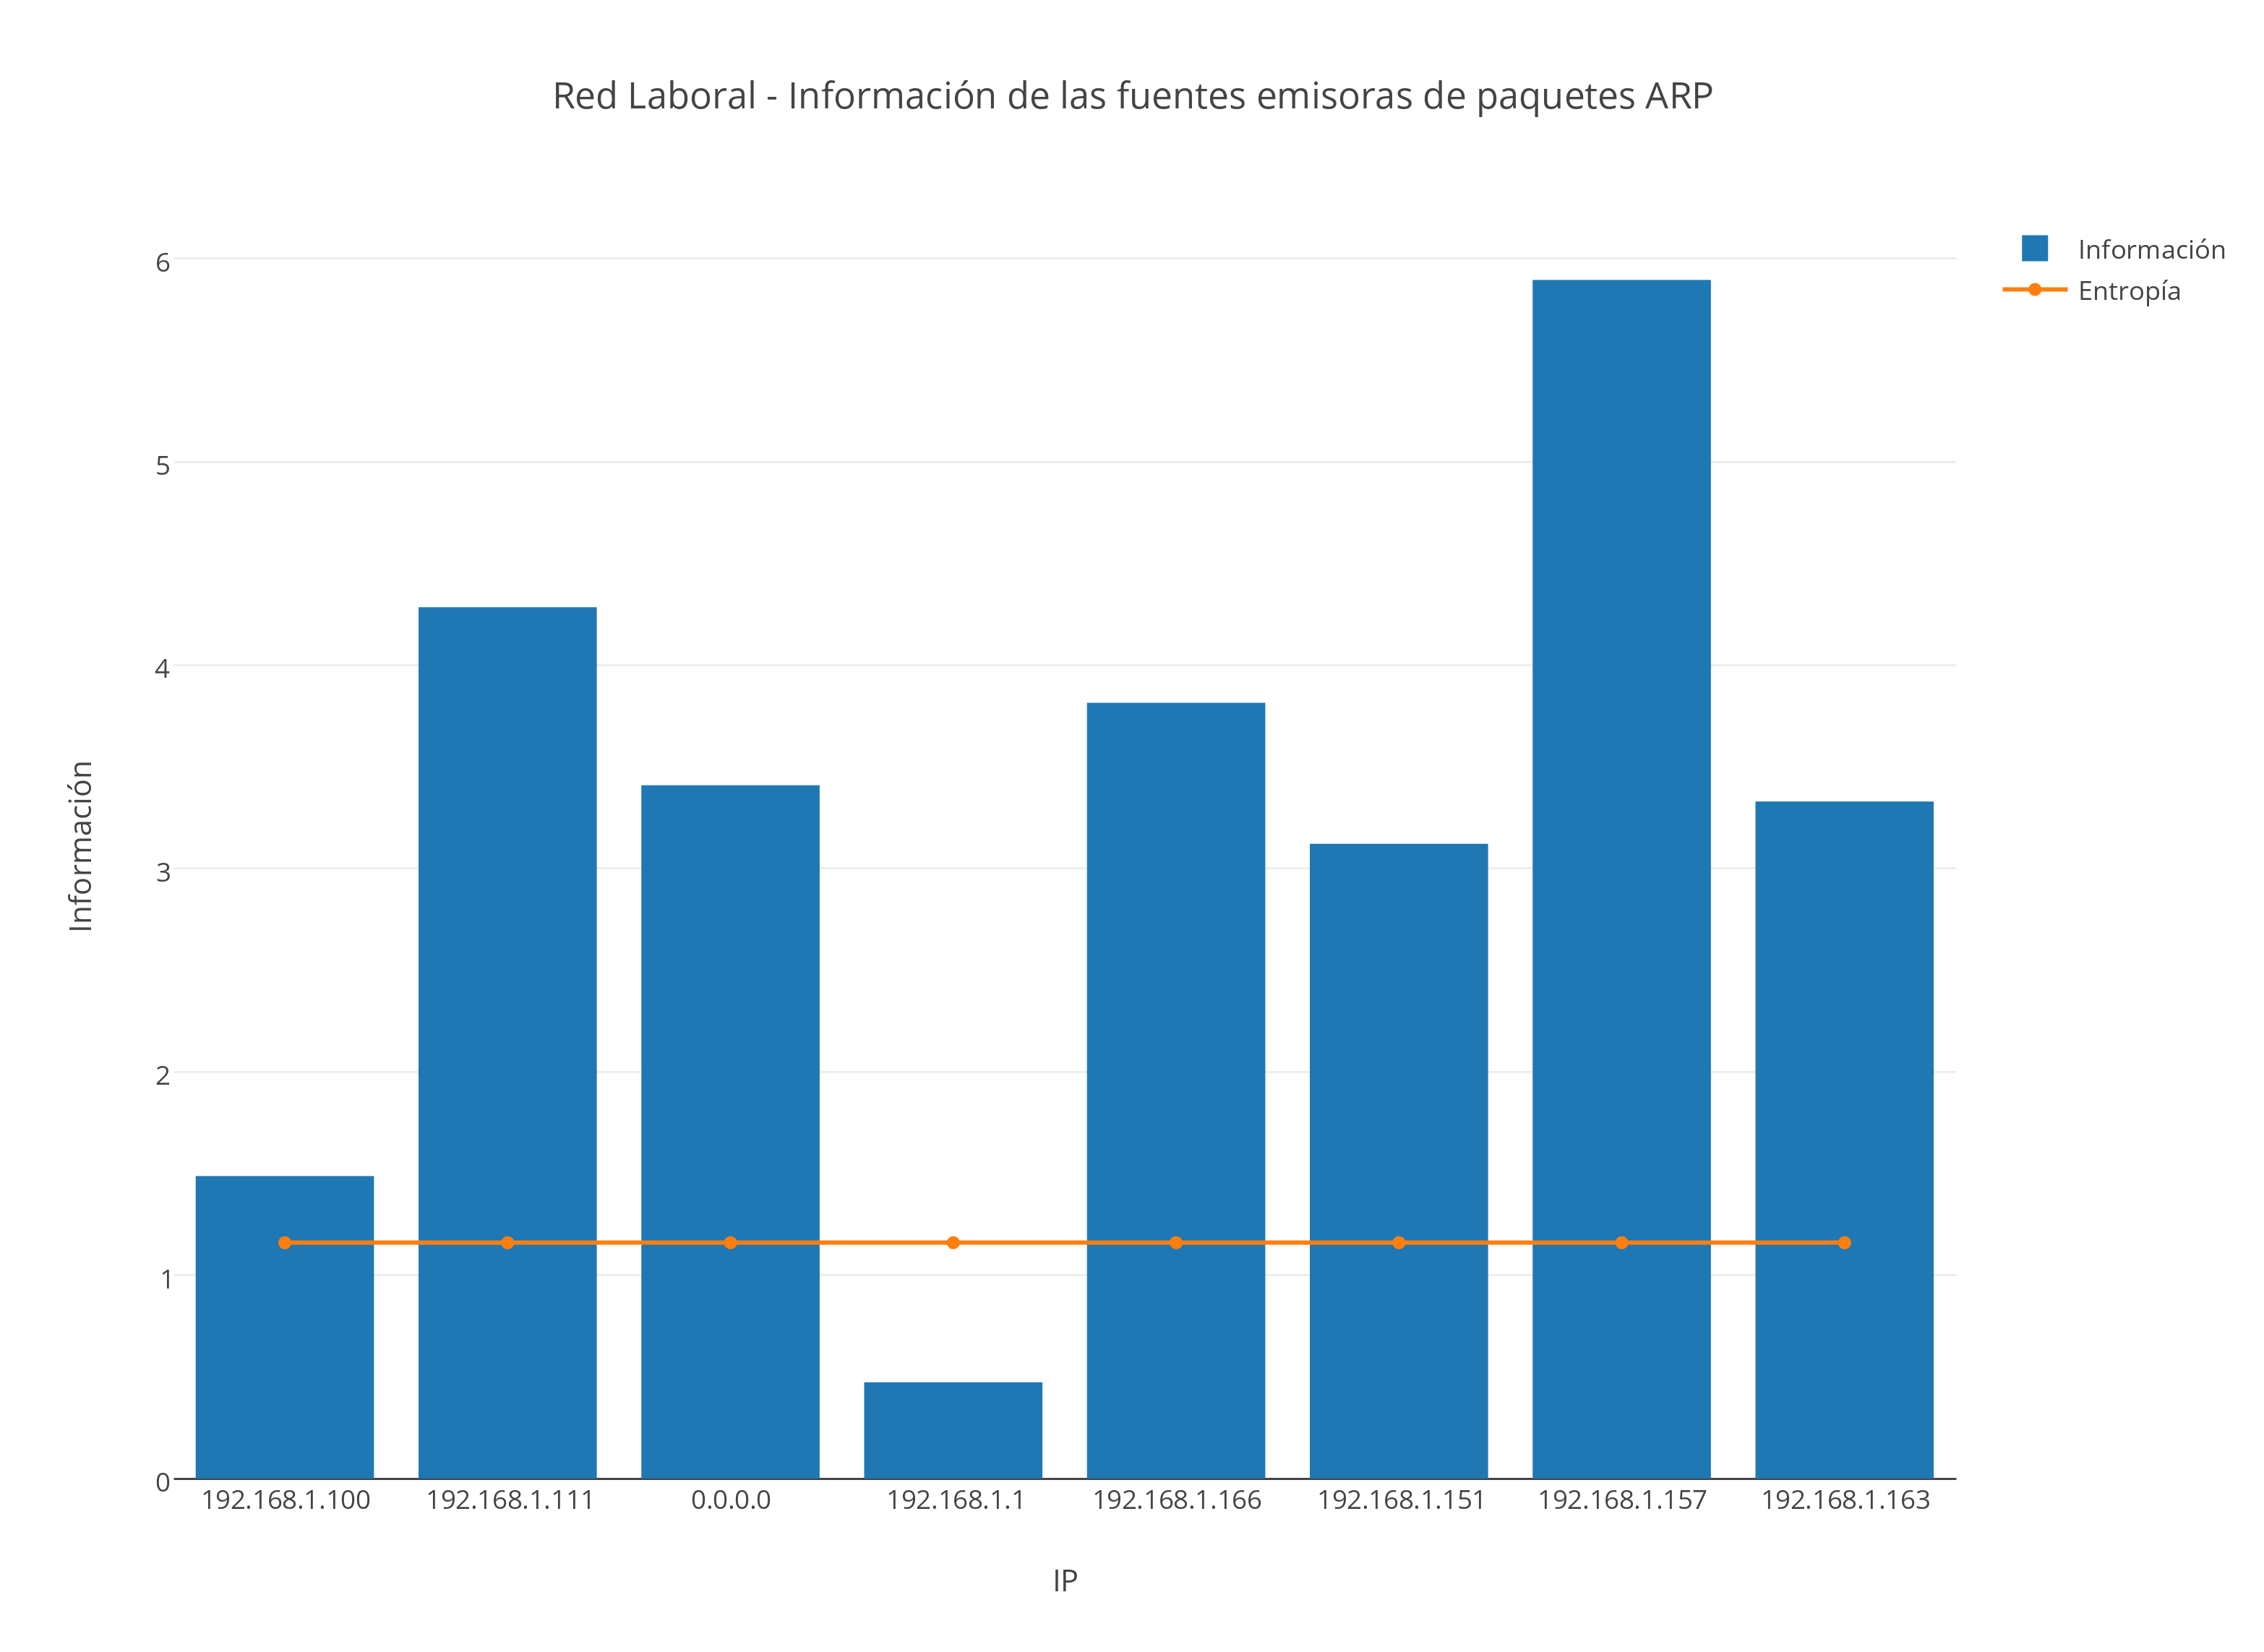
\includegraphics[width=400pt]{img/RedLaboralFuentesEmisorasARP}
    \caption{}
    \label{laboralEmisoras}
\end{figure}

Dentro de las IPs emisoras se puede destacar la participaci\'on activa de el nodo 192.168.1.1, la cu\'al aporta un valor muy pequeño de informaci\'on, encontr\'andose por debajo de la entrop\'ia. Esto indicar\'ia que se trata del host que m\'as paquetes ARP env\'ia dentro de la red - y esto es correcto, ya que en efecto es el nodo 4, el nodo correspondiente al router.\\

\begin{figure}[h!]
    \centering                                                       
    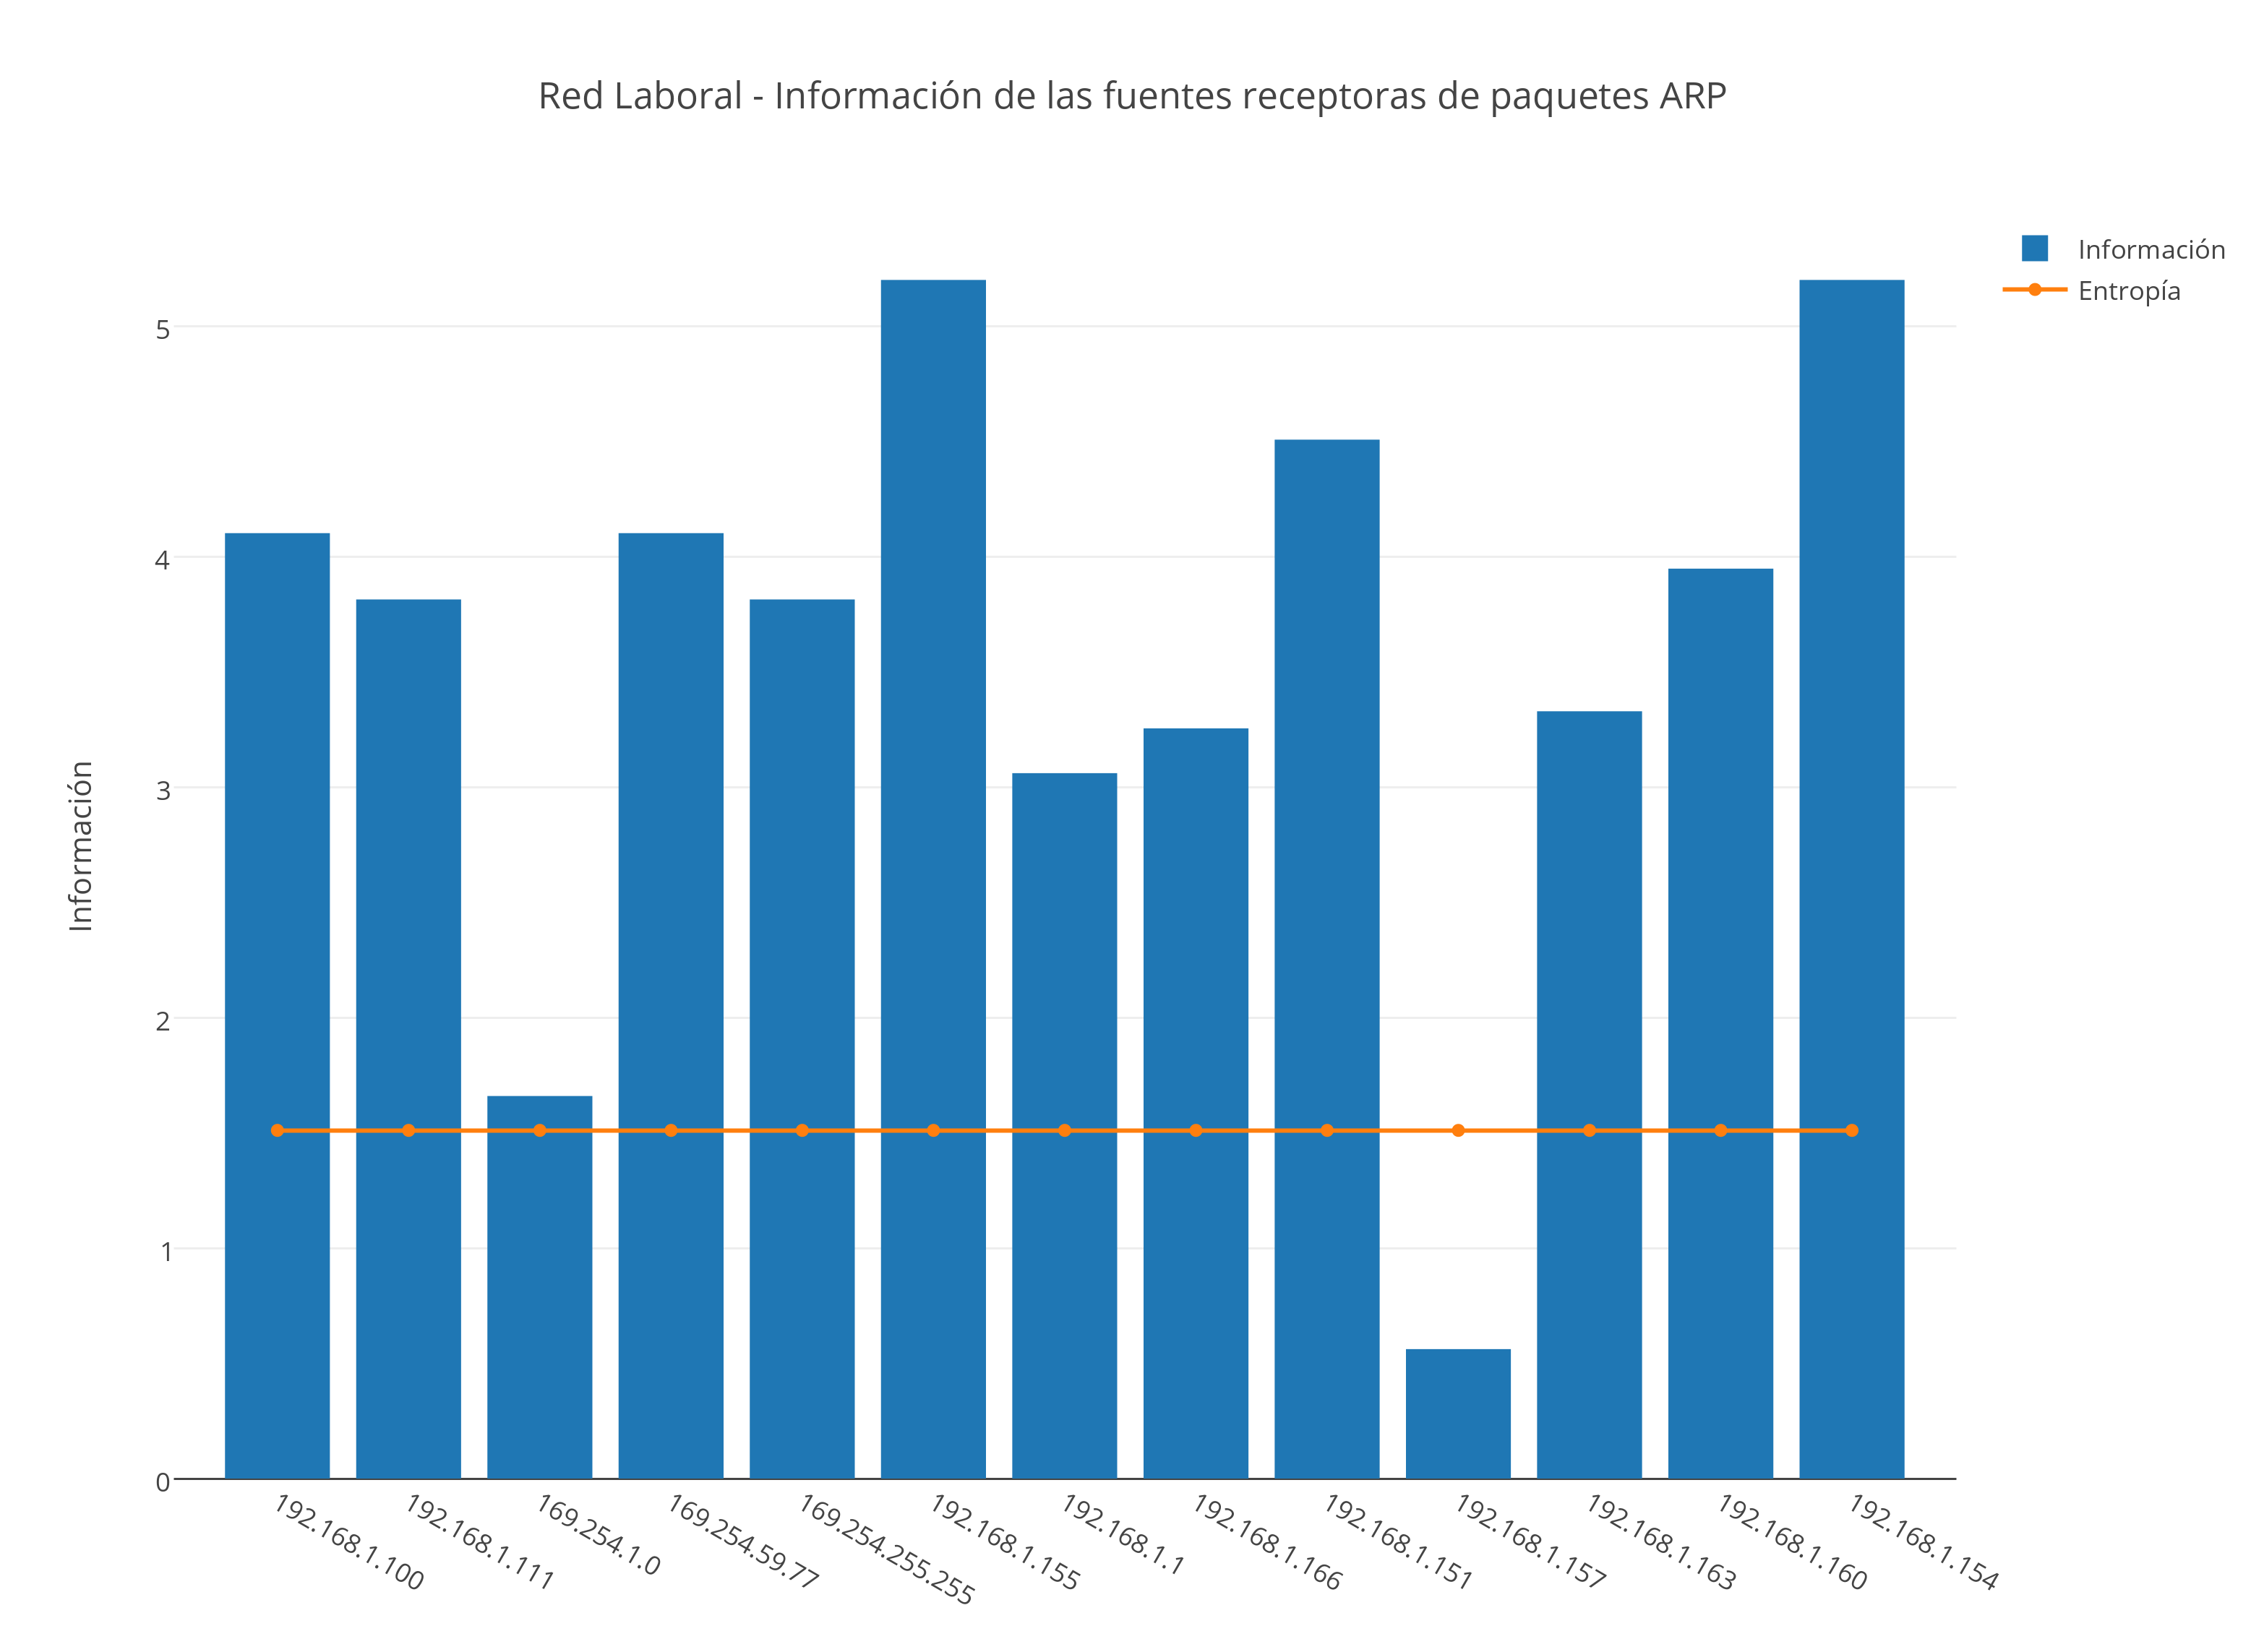
\includegraphics[width=400pt]{img/RedLaboralFuentesReceptorasARP}
    \caption{}
    \label{laboralReceptoras}
\end{figure}

Si lo buscamos en el gr\'afico \ref{laboralReceptoras}, el mismo nodo aporta una informaci\'on por encima de la media, pero sin ser destacada. Es decir, que hay nodos que env\'ian m\'as paquetes que el router. Esto es porque, si bien el router es salida de todos los nodos a internet, las conexiones internas (es decir, entre nodos, con el servidor local, por ejemplo) tienen m\'as peso, y se usan esas conexiones m\'as que la red externa.\\

Otro caso a destacar es el de la IP 192.168.1.157 (nodo 7). Compar\'andolo en ambos gr\'aficos, se lo ve como el punto m\'aximo en uno y el m\'inimo en otro: el nodo 7 es aquel que m\'as paquetes env\'ia y el que m\'as recibe, conect\'andose tanto con el router como con el servidor local. Si bien no pudimos verificar la identidad de dicha IP (pues utilizamos \textit{NAT} para ciertas IPs y esta cae en una de ellas, siendo imposible identificar cu\'al era su identidad al momento de la medici\'on), parece sensato suponer que se debe a un nodo (computadora) trabajando con el servidor y el router a la vez, pudiendo deberse la gran cantidad de paquetes enviado por estar subiendo/copiando material a uno de ellos.\\

\newpage
\subsection{Red Bonafide}
 Por \'ultimo, dadas las peque\~nas dimensiones de las redes anteriores, decidimos tomar datos de la red p\'ublica ofrecida por el local Bonafide. La captura se realiz\'o por un lapso de media hora en modo promiscuo.

\subsubsection{Nodos intervinientes}

En el gr\'afico \ref{bonafideGraph} se pueden ver los resultados de obtenidos.

\begin{figure}[h!]
    \centering                                                       
    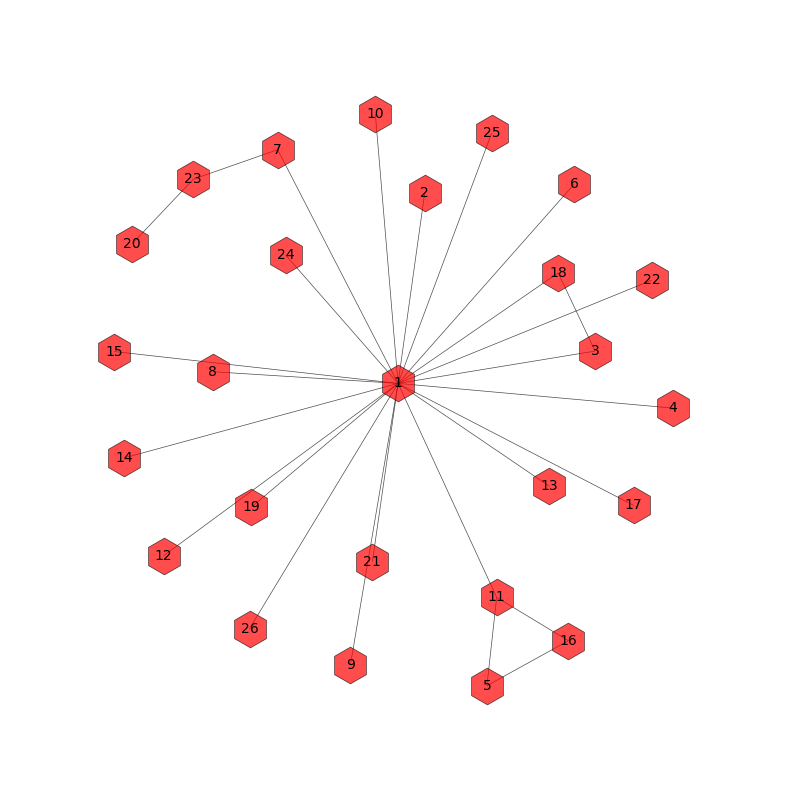
\includegraphics[width=400pt]{img/bonafideGraph.png}
    \caption{Grafo de Red Bonafide}
    \label{bonafideGraph}
\end{figure}
Si bien el grafo resultante no es exactamente la idea previa que ten\'iamos de \'el (un grafo estrella con el nodo root como ra\'iz) resulta interesante observar la indiscutible predominancia de aristas incidentes al nodo 1, descripto con la direcci\'on IP 192.168.1.1: el resto de los nodos son adyacentes a \'el o tienen un camino al mismo de - a lo sumo - tercer grado.\\
Consideramos que estos datos son suficientes como para deducir que dicha direcci\'on IP coincide con la del router.\\
Al indagar acerca de la naturaleza de los \'unicos nodos que no se encuentran conectados de forma directa al nodo 1 (el 5 (192.168.1.110), el 16 (192.168.1.4), el 23(0.0.0.0) y el 20 (169.254.201.232)) llegamos a las siguientes conclusiones: \\
\begin{itemize}
	\item Tanto el nodo 5 como el 16 (ambos de clase C) se comunican con el router a trav\'es del nodo 11 (192.168.1.105). Ahondando en las caracter\'isticas de estas transferencias, se puede ver que el nodo 11 realiza requests a los nodos 1, 5 y 16, pero s\'olo llega a \'el un request desde el nodo 16. Podr\'iamos entonces inferir que el nodo 11 puede estar funcionando como switch.
	\item El nodo 20 se conecta al 23 y \'este \'ultimo al 7 (192.168.1.100). Esto forma la secuencia 169.254.201.232 (clase B)- 0.0.0.0 - 192.168.1.100 (clase C) - router. Si bien no se trata de un grafo dirigido, se puede ver en los resultados que la direcci\'on 0.0.0.0 nunca recibe datos que podamos escuchar, si no que env\'ia requests a ambos nodos que lo circundan.\\ De acuerdo a lo investigado, inferimos que se trata de un fen\'omeno que ocurre cuando un nuevo host se conecta a la IP, con el fin de verificar que no tenga una direcci\'on que se encuentre en uso, evitando as\'i las IP duplicadas.\\
\end{itemize}


\subsubsection{Frecuencia de los distintos tipos de paquetes}

En el gr\'afico \ref{bonafidePaquetes} se pueden ver los resultados de obtenidos.

\begin{figure}[h!]
    \centering                                                       
    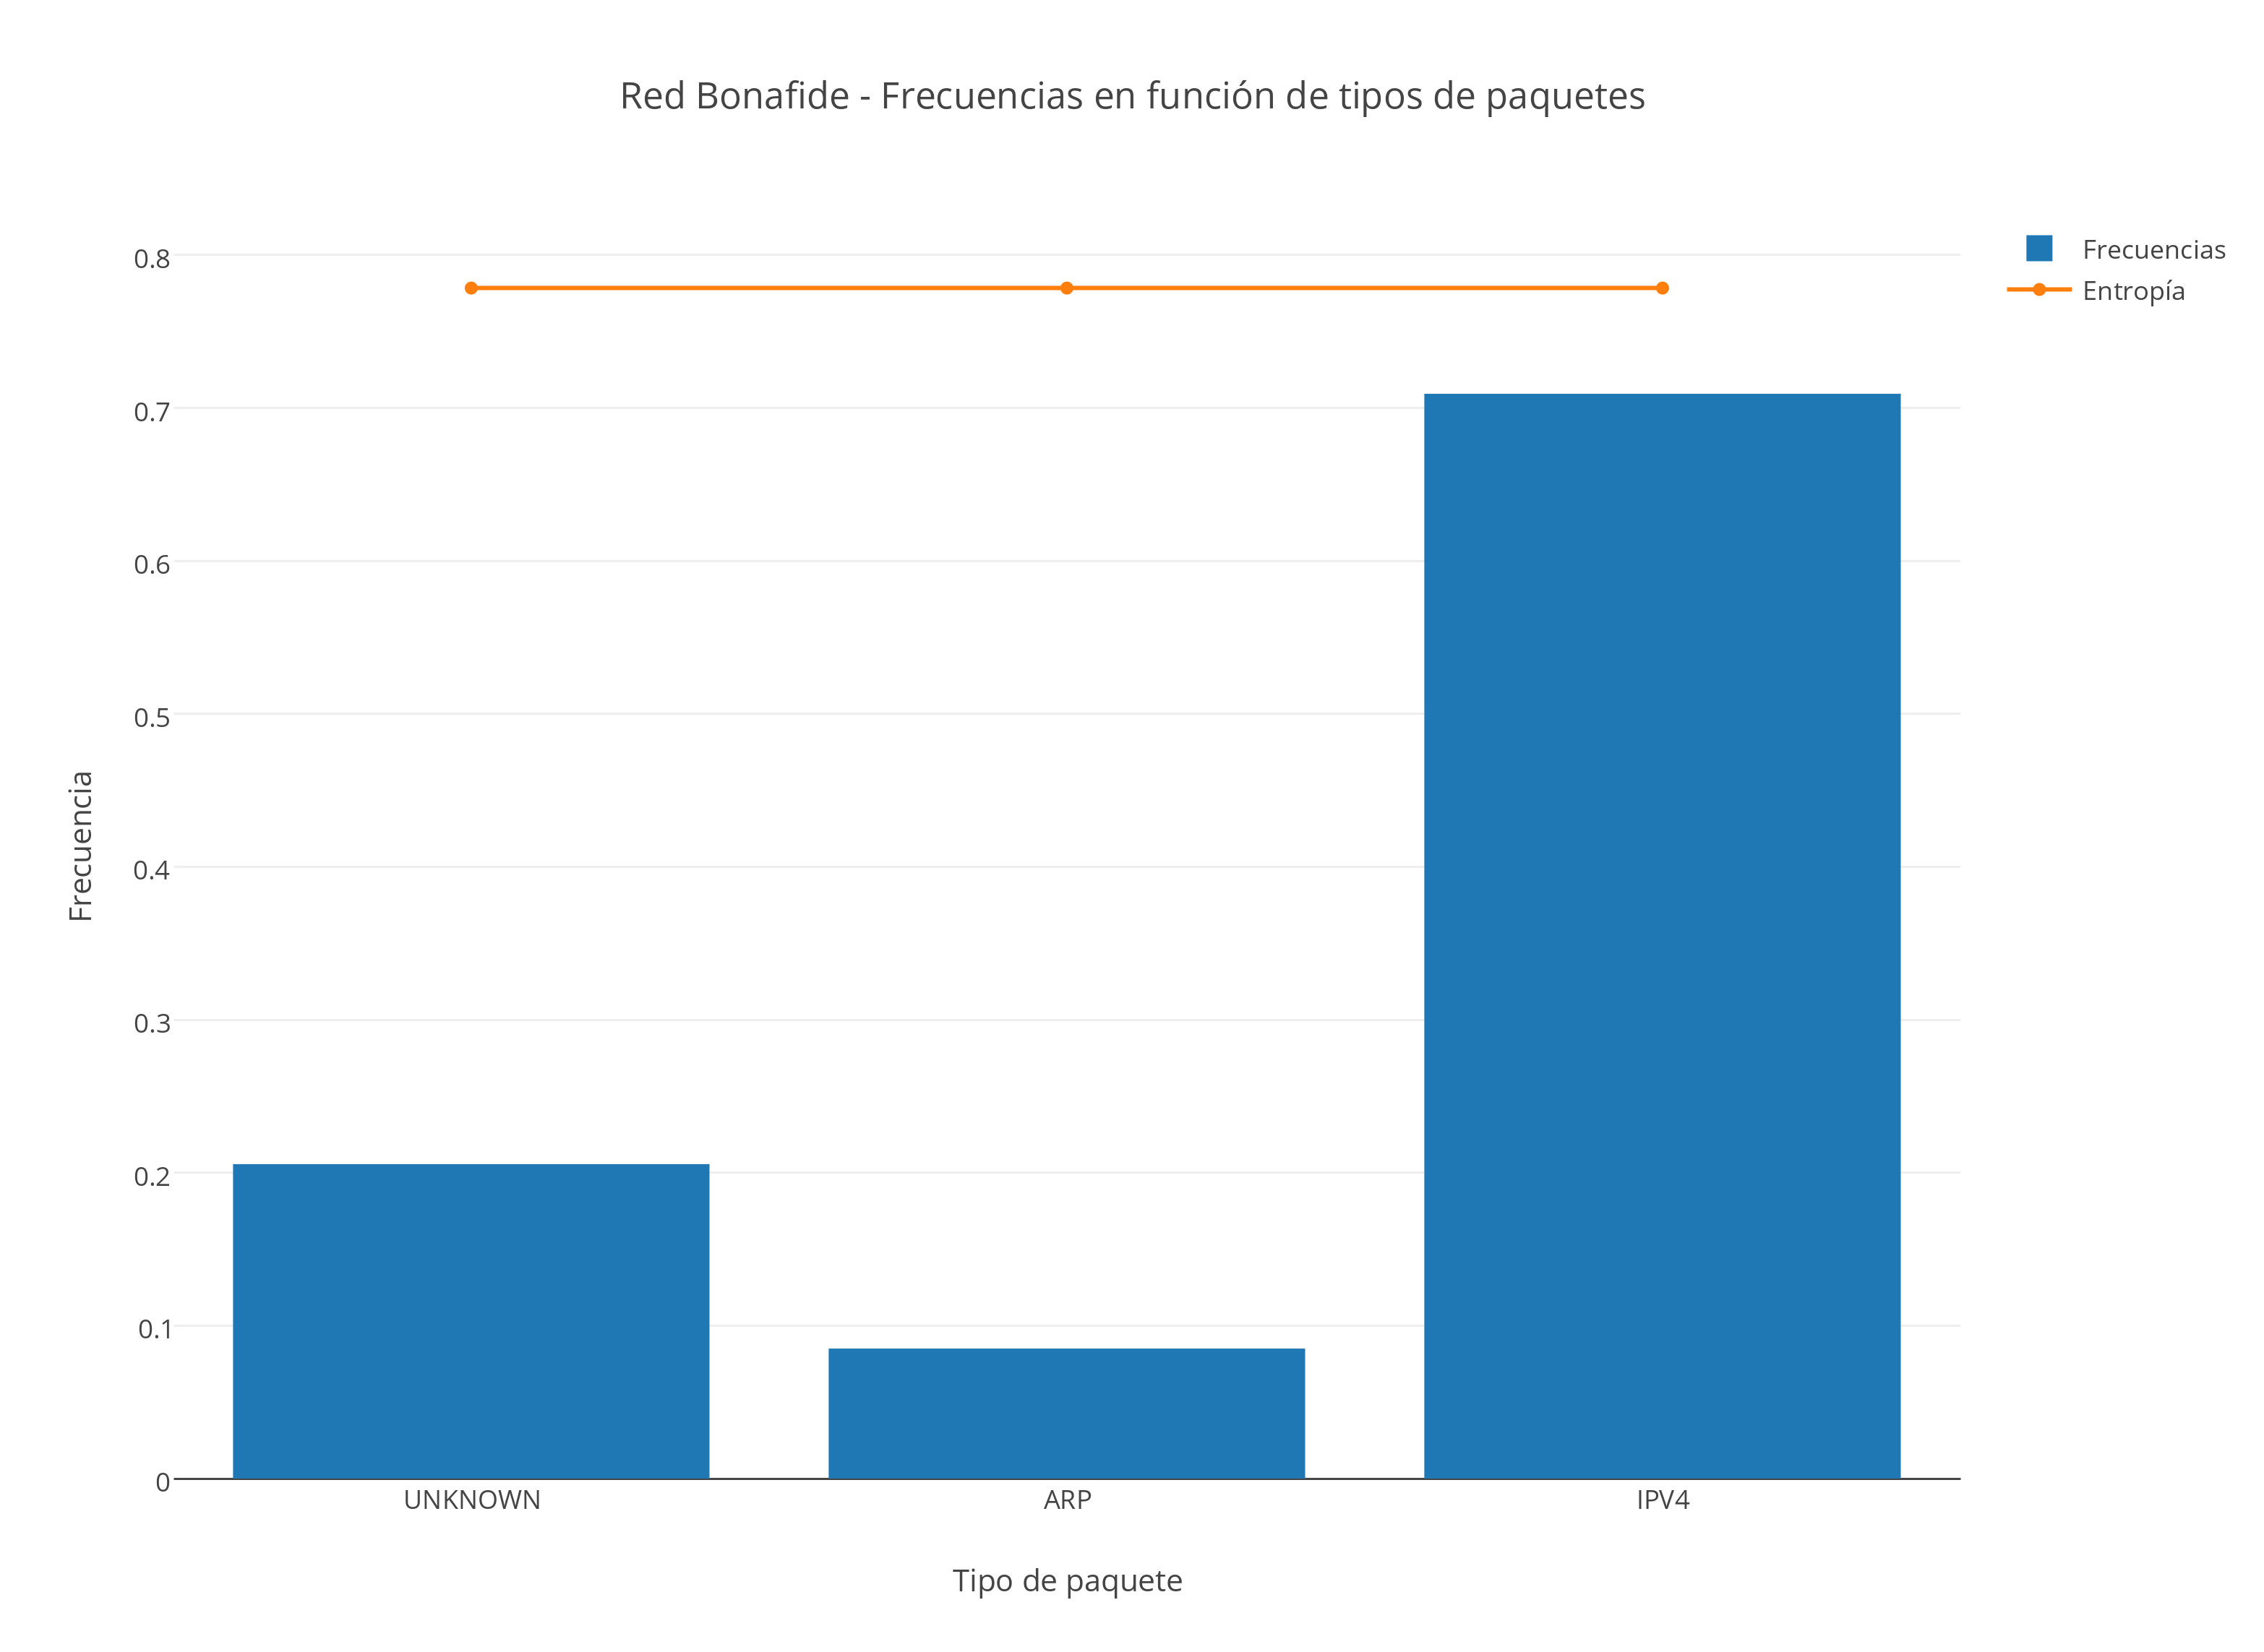
\includegraphics[width=400pt]{img/BonafideFrecuenciaVsTipoPaquetes}
    \caption{}
    \label{bonafidePaquetes}
\end{figure}

En este caso se ve una amplia predominancia de los paquetes de tipo IPv4. Esto se corresponde con nuestras expectativas, puesto que los paquetes de tipo ARP se envían como forma de reconocimiento entre dispositivos. Una vez que estos reconocimientos fueron establecidos, el caudal de paquetes de transferencia IPv4 aumenta, superando así a los paquetes ARP en una red quya estructura no se modifica a cada momento debido a la conexión y desconexión de dispositivos.

\subsubsection{Informaci\'on de las fuentes emisoras y receptoras de paquetes ARP.}

\begin{figure}[h!]
    \centering                                                       
    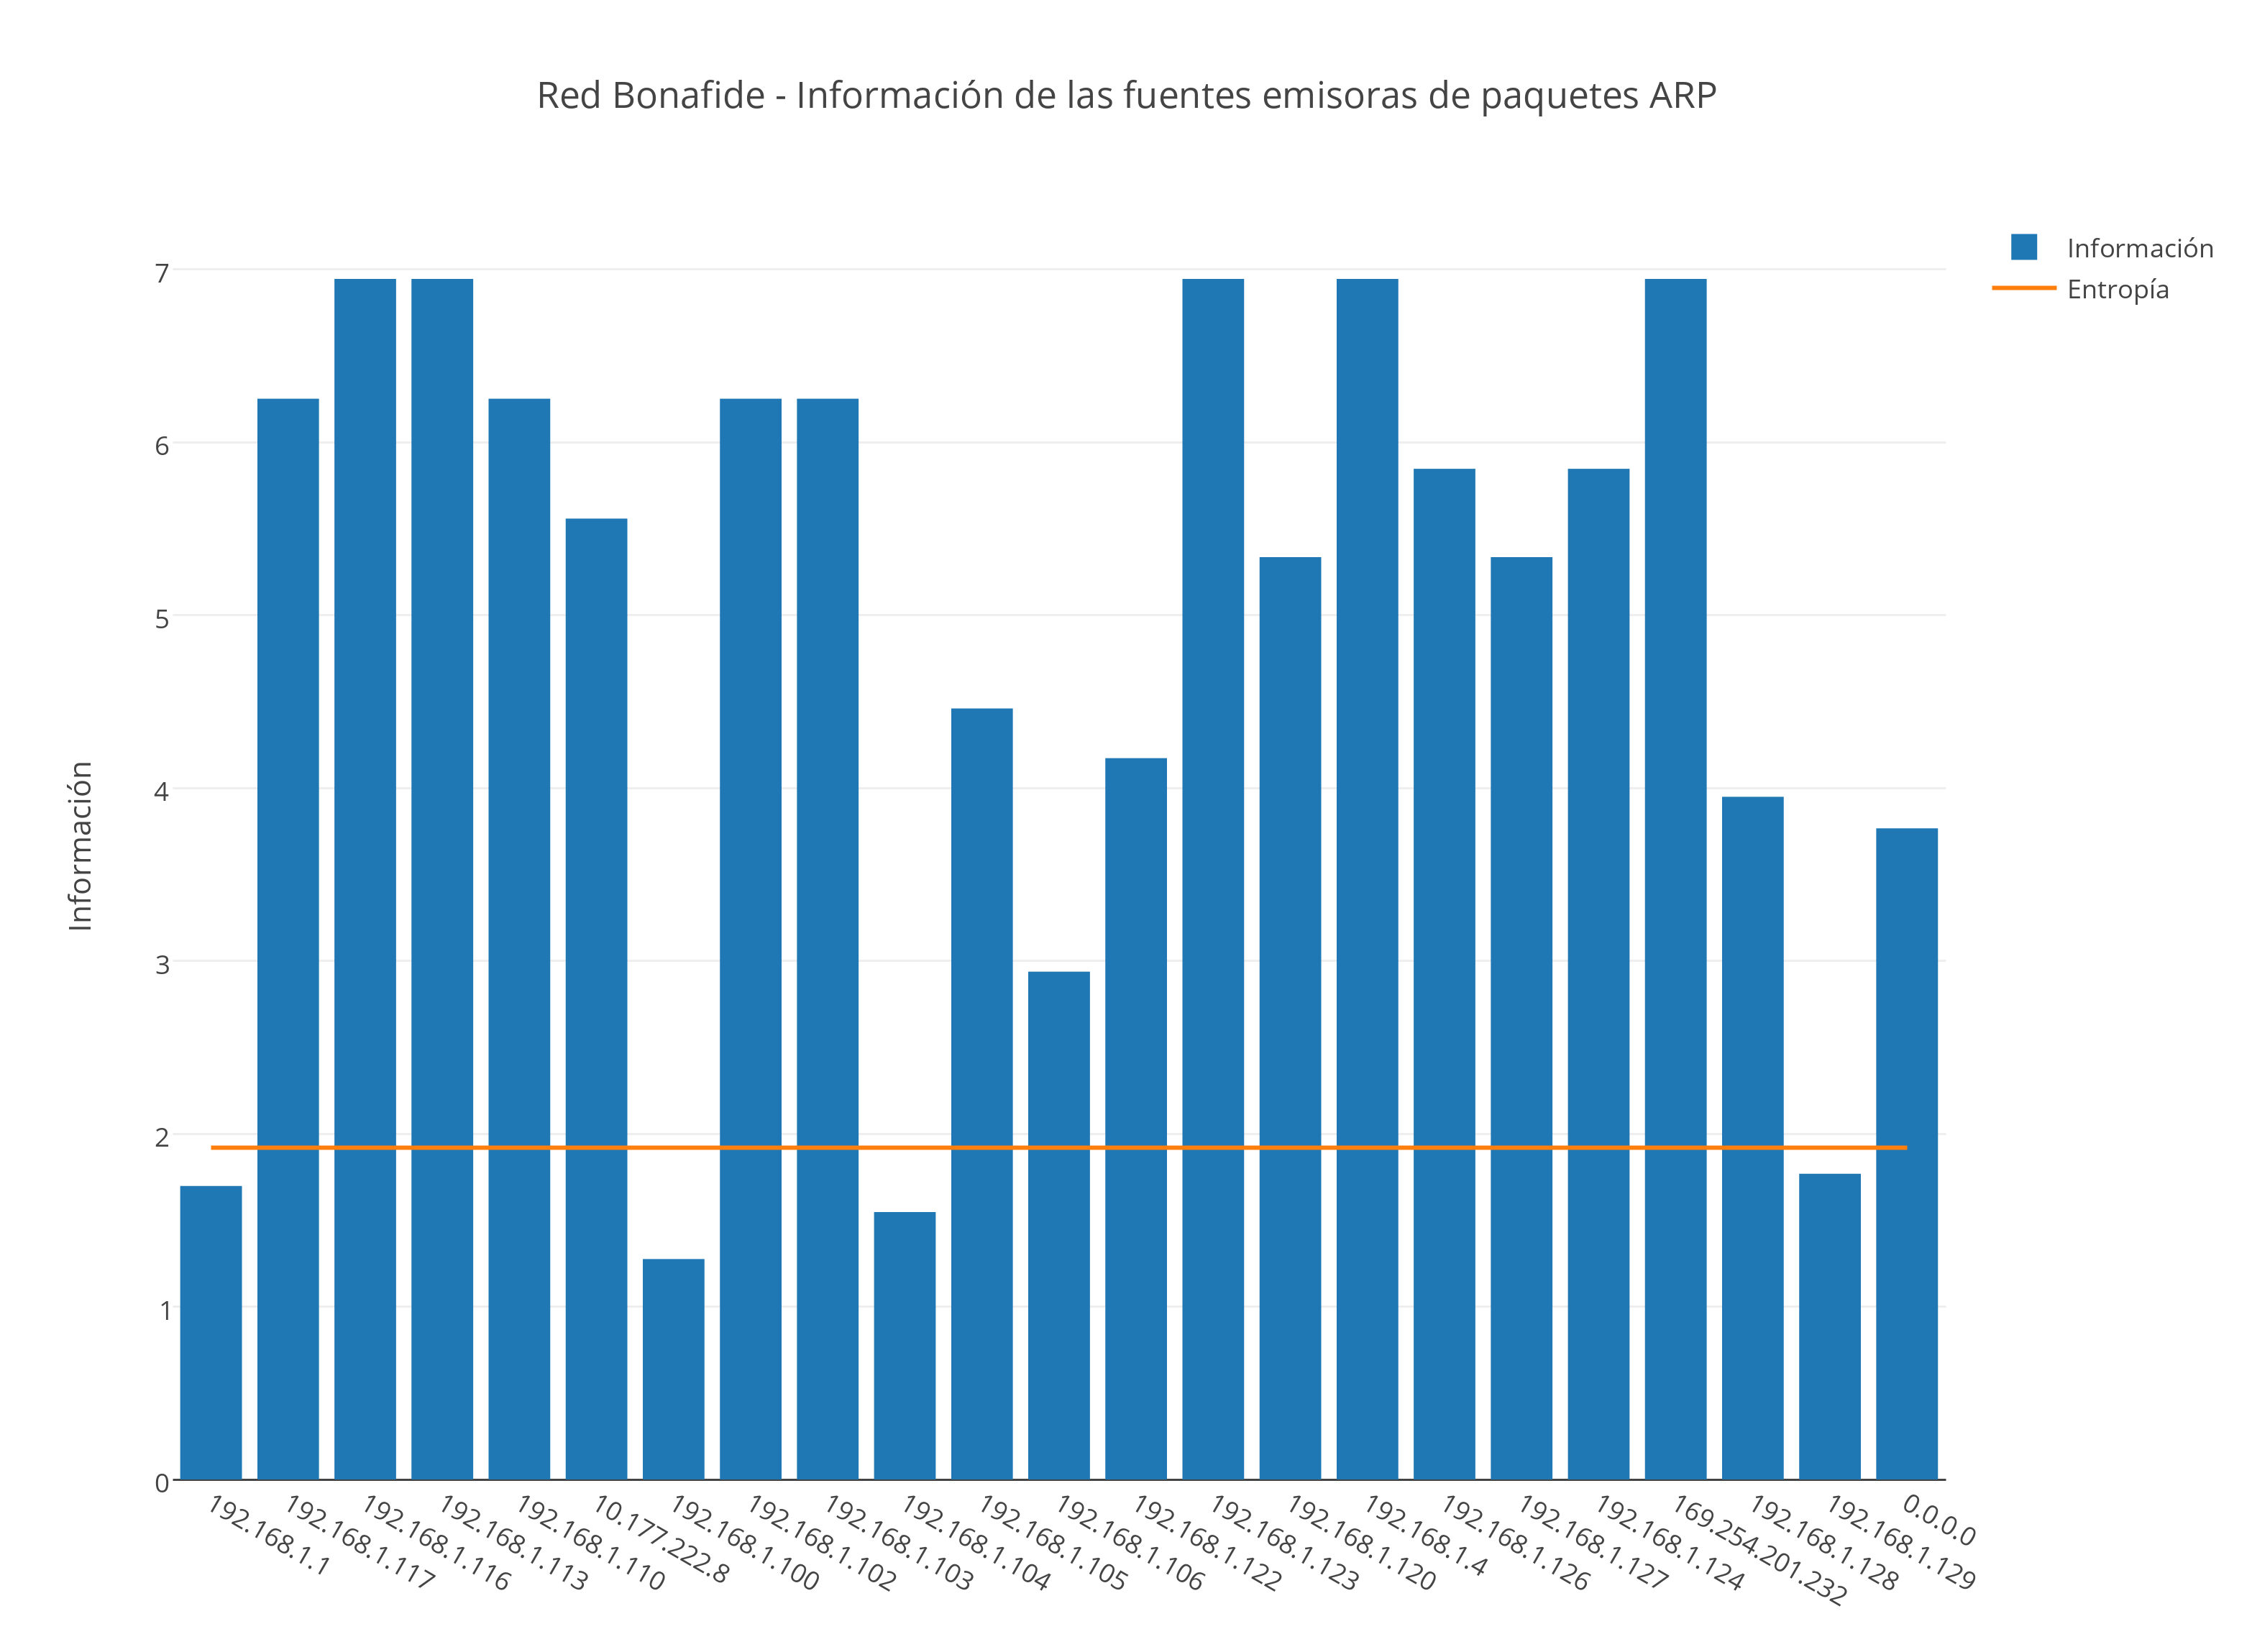
\includegraphics[width=400pt]{img/RedBonafideFuentesEmisorasARP}
    \caption{}
    \label{bonafideEmisoras}
\end{figure}

\begin{figure}[h!]
    \centering                                                       
    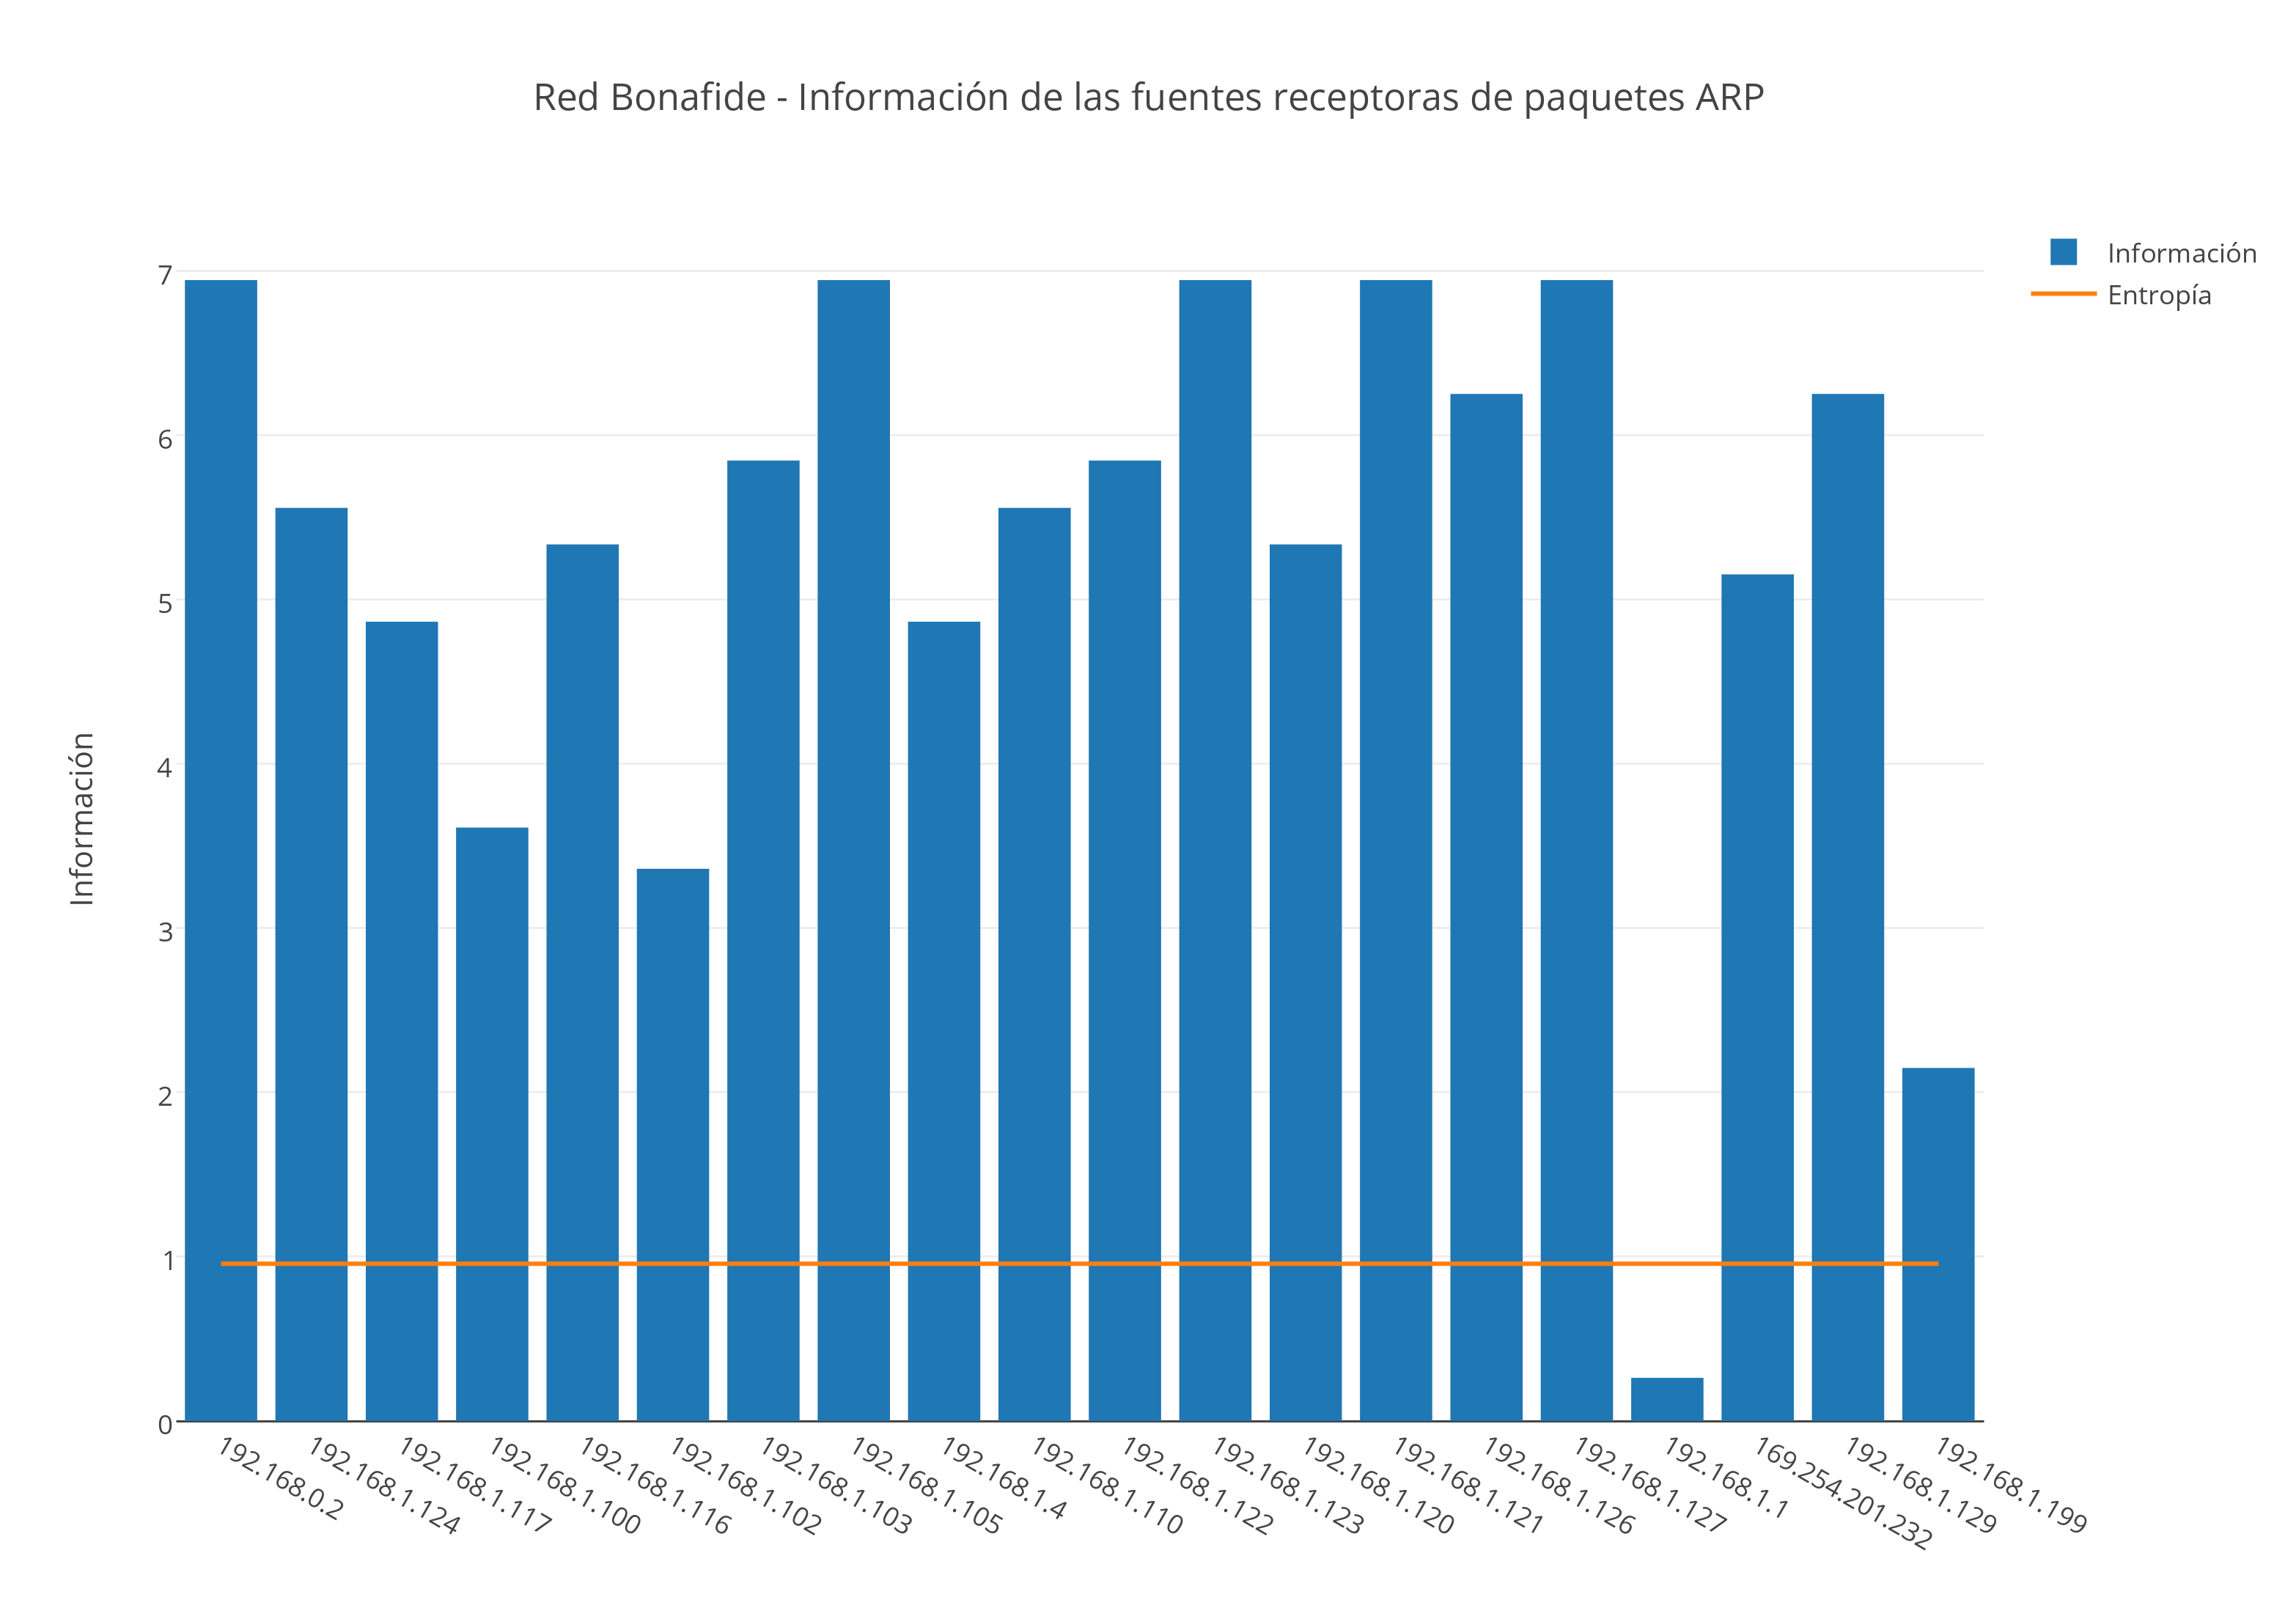
\includegraphics[width=400pt]{img/RedBonafideFuentesReceptorasARP}
    \caption{}
    \label{bonafideReceptoras}
\end{figure}

Este caso podr\'ia ser el de m\'as arduo an\'alisis, puesto que es el que mayor caudal de datos presenta. Sin embargo, la gran cantidad de informaci\'on que contiene facilita la distinci\'on de los nodos significativos. \\`
Como se puede observar en la figura \ref{bonafideEmisoras}, hay cuatro nodos que merecen nuestro reconocimiento: el 7 (192.168.1.100), el 10 (192.168.1.104), el 1 (192.168.1.1) y el 22 (192.168.1.129). Estos aportan un nivel de informaci\'on menor al valor de la entrop\'ia, indicando, en este caso, que se encuentran enviando una gran cantidad de parquetes ARP. Esta deducci\'on no se podr\'ia haber hecho analizando \'unicamente el grafo que representa la red, dado que all\'i tres de dichos nodos no parecen destacarse de los dem\'as.\\

En cambio, en la figura \ref{bonafideReceptoras}, se refuerza fuertemente lo que se percibe en el grafo de la imagen \ref{bonafideGraph}: La mínima informaci\'on est\'a vinculada a la IP 192.168.1.1, es decir, al nodo identificado con el n\'umero 1. Con los tres gr\'aficos presentados en conjunto es posible concluir que la IP 192.168.1.1 es la que identifica al router, no s\'olo por la cantidad de paquetes ARP que env\'ia y recibe sino tambi\'en por la estructura de la red que se conforma en torno al dispositivo.


\section{Conclusiones}

Al comenzar a resolver los problemas presentados ten\'iamos una idea poco pulida acerca de las redes en general. Conjetur\'abamos ideas respecto a sus estructuras y comportamientos que se vieron refutadas durante el desarrollo y an\'alisis del presente trabajo pr\'actico. Por poner un ejemplo, esper\'abamos encontrar redes cuyo grafo fuese un \'arbol estrella, con el centro como Router y donde no hubiese ciclos ni conexi\'on alguna entre los nodos secundarios. Asimismo, hicieron su aparici\'on direcciones IP que no ten\'iamos presentes.\\
Luego de concretar los experimentos realizados presentamos sus resultados de una forma que consideramos apropiada estudiamos sus resultados, destacando nodos que consideramos distinguidos, investigando el motivo de los resultados imprevistos, obteniendo datos (como la informaci\'on de diversos eventos y la entrop\'ia de una variada cantidad de fuentes) y reuniendo para el an\'alisis integral los datos proporcionados por distintas herramientas que generamos.\\
Luego de todo este proceso, concluimos que:
\begin{itemize}
	\item el c\'alculo de la entrop\'ia resulta imprescindible para conocer la predictibilidad de la fuente que se estudia. 
	\item Es posible deducir con cierta confianza cu\'al es el Router de una red a partir de las interacciones en las que se involucra pasiva o activamente cada host: es, generalmente, el que mayor actividad tiene por su alta intervenci\'on como mediador entre m\'aquinas.
    \item El protocolo ARP es fundamental para la traducci\'on entre direcciones de nivel de red (IP) y direcciones de nivel de enlace (MAC).  
\end{itemize}
